

\documentclass[a4paper]{article} 

\usepackage[a4paper, margin=1cm, top=1cm, bottom=1cm, left=1.5cm, right=1.5cm]{geometry}

\setlength{\parskip}{0pt}
\setlength{\parindent}{0in}

%----------------------------------------------------------------------------------------
%	PACKAGES AND OTHER DOCUMENT CONFIGURATIONS
%----------------------------------------------------------------------------------------

\usepackage{blindtext} % Package to generate dummy text
\usepackage{charter} % Use the Charter font
\usepackage[utf8]{inputenc} % Use UTF-8 encoding
\usepackage{microtype} % Slightly tweak font spacing for aesthetics
\usepackage[english, spanish, es-nodecimaldot]{babel} % Language hyphenation and typographical rules
\usepackage{amsthm, amsmath, amssymb} % Mathematical typesetting
\usepackage{multicol}
\usepackage{float} % Improved interface for floating objects
\usepackage[final, colorlinks = true, 
            linkcolor = black, 
            citecolor = black]{hyperref} % For hyperlinks in the PDF
\usepackage{graphicx, multicol} % Enhanced support for graphics
\usepackage{xcolor} % Driver-independent color extensions
\usepackage{marvosym, wasysym} % More symbols
\usepackage{rotating} % Rotation tools
\usepackage{censor} % Facilities for controlling restricted text
\usepackage{listings, style/lstlisting} % Environment for non-formatted code, !uses style file!
\usepackage{pseudocode} % Environment for specifying algorithms in a natural way
\usepackage{style/avm} % Environment for f-structures, !uses style file!
\usepackage{booktabs} % Enhances quality of tables
\usepackage{tikz-qtree} % Easy tree drawing tool
\usepackage{enumitem}  
\usepackage{graphicx} 
\usepackage{booktabs}
\usepackage{array}  
\usepackage{bm}
\tikzset{every tree node/.style={align=center,anchor=north},
         level distance=2cm} % Configuration for q-trees
\usepackage{style/btree} % Configuration for b-trees and b+-trees, !uses style file!
\usepackage[backend=biber,style=numeric,
            sorting=nyt]{biblatex} % Complete reimplementation of bibliographic facilities
\addbibresource{sample.bib}
\usepackage{csquotes} % Context sensitive quotation facilities
\usepackage[yyyymmdd]{datetime} % Uses YEAR-MONTH-DAY format for dates
\renewcommand{\dateseparator}{-} % Sets dateseparator to '-'
\usepackage{fancyhdr} % Headers and footers
\pagestyle{fancy} % All pages have headers and footers
\fancyhead{}\renewcommand{\headrulewidth}{0pt} % Blank out the default header
\fancyfoot[L]{} % Custom footer text
\fancyfoot[C]{} % Custom footer text
\fancyfoot[R]{\thepage} % Custom footer text
\newcommand{\note}[1]{\marginpar{\scriptsize \textcolor{red}{#1}}} % Enables comments in red on margin
\DeclareMathOperator*{\plim}{plim}
\usepackage[most]{tcolorbox}
\usepackage{cancel}
\usepackage{adjustbox}
\addto\captionsspanish{
\def\listtablename{\'Indice de tablas}%
\def\tablename{Tabla}}
\usepackage{xcolor}
\usepackage{multirow}
\usepackage{listings}
\usepackage{bbm}
\newcommand{\indep}{\perp\!\!\!\!\perp} 
\definecolor{myblue}{RGB}{0,163,243}
\definecolor{moradito}{RGB}{63,1,143}

\usepackage{tcolorbox}
\newtcolorbox{solucion}{colbacktitle=gray, coltitle=white, breakable,
colframe=black, colback=white, fonttitle=\bfseries,parbox=true,
title=Solución:}
\usepackage{float}

\usepackage{listings,xcolor}
\usepackage{upquote}
 
\usepackage[spanish]{babel}
\usepackage{enumerate}
\usepackage{hyperref} 
%\decimalpoint
\setlength\parindent{0pt}
\newcommand*{\QED}{\hfill\ensuremath{\blacksquare}}
\usepackage{authblk}
\selectlanguage{spanish}

\newtheorem{theorem}{Teorema}[section]
\newtheorem{corollary}{Corolario}[theorem]
\newtheorem{lemma}[theorem]{Lema}
\theoremstyle{remark}
\newtheorem*{remark}{Considere}
\DeclareUnicodeCharacter{2212}{-}
\usepackage{epigraph}

%\usepackage[natbibapa]{apacite}
\usepackage{tikz}
\usepackage{physics}
\newcommand{\ubar}[1]{\text{\b{$#1$}}}

\usepackage{tcolorbox}


\usepackage{float}

\usepackage{listings,xcolor}
\usepackage{upquote}
\usepackage{subfigure}

 
\theoremstyle{definition}
\newtheorem{definition}{Definición}[section]

\usepackage{listings}
\usepackage{xcolor}

% Configuración para resaltar código MATLAB
\lstset{
    language=Matlab, % Indica el lenguaje para resaltar
    basicstyle=\ttfamily\small, % Estilo básico del texto
    keywordstyle=\color{blue}, % Estilo para palabras clave
    commentstyle=\color{green}, % Estilo para comentarios
    stringstyle=\color{red}, % Estilo para cadenas de texto
    numberstyle=\tiny\color{gray}, % Estilo para números de línea
    stepnumber=1, % Incremento entre números de línea
    numbersep=10pt, % Espacio entre números y código
    backgroundcolor=\color{white}, % Color de fondo del código
    showstringspaces=false, % Evitar espacios para cadenas de texto
    breaklines=true, % Permitir líneas largas se corten
    frame=single, % Crear un borde alrededor del bloque de código
}


%Código para imágenes
%\begin{figure}[H]
%\centering
%\includegraphics[scale=0.5]{PIB.png}
%\caption{Crecimiento porcentual del PIB desde 1990 hasta 2009}
%\end{figure}

\usepackage{amsmath}
\usepackage[utf8]{inputenc}
\usepackage[spanish]{babel}
\usepackage{amsmath}
\usepackage{amsfonts}
\usepackage{amssymb}
\usepackage{hyperref}


\title{Big Data y Machine Learning: Problem Set 3}
\author{Ignacio Sarmiento}
\date{1 de Diciembre de 2024}
\begin{document}
\maketitle
\begin{center}

\begin{tabular}{ c c c }
 \textbf{Integrantes:} & Juliet Alejandra Molano Rizo & 202226070 \\
 & Henry Nicolas Carvajal Cardenas & 201718787\\
 & Diego Fernando Cuesta Mora & 202315672\\
 & Jorge Ramirez Sanchez & 202116747
\end{tabular}

\end{center}

%-------------------------------------------------%
\section{Introducción} \\

Predecir con precisión los precios de viviendas es esencial para un mercado inmobiliario sostenible, ya que facilita decisiones informadas para compradores, vendedores e inversionistas, reduce la especulación y promueve una valoración justa de los inmuebles. Sin embargo, fallas en los modelos predictivos pueden tener consecuencias significativas, como ocurrió con la empresa Zillow. En un esfuerzo por automatizar la compra y venta de propiedades, Zillow implementó algoritmos de predicción que sobrestimaron el valor de las viviendas, lo que ocasionó pérdidas financieras de 500 millones de dólares y una reducción del 25\% de su fuerza laboral. Este ejemplo destaca la importancia de diseñar modelos robustos que minimicen los errores y capturen las dinámicas complejas del mercado. El precio de una vivienda no es únicamente el reflejo de sus características físicas, como el área o el número de habitaciones. Según Rosen (1974), los precios de los bienes diferenciados están influenciados por un conjunto de atributos intrínsecos (estructura) y extrínsecos (ubicación, proximidad a servicios), lo que se conoce como 'precios hedónicos'. Este enfoque ha sido ampliamente utilizado en el análisis de mercados inmobiliarios, proporcionando un marco teórico que permite capturar las complejidades asociadas a la interacción entre las características de las propiedades y su entorno.\\

En Bogotá, el rápido crecimiento poblacional y la alta demanda de vivienda, especialmente en localidades como Chapinero donde la oferta es limitada y los usos del suelo son diversos, generan complejidad en el mercado. La falta de herramientas precisas para estimar precios puede aumentar la volatilidad y profundizar desigualdades en el acceso a la vivienda. Estudios como el de Nieto (2022) destacan la importancia de incluir variables como el estado de las vías, el diseño arquitectónico y el estrato socioeconómico, mientras que investigaciones recientes, como la de Sicilia Gómez (2024), resaltan la incorporación de variables contextuales y textuales para mejorar la precisión en las predicciones.\\

\textbf{Antecedentes} \\

En Colombia, diversos estudios han explorado las dinámicas del mercado inmobiliario mediante modelos de aprendizaje automático. En Bogotá, Nieto (2022) desarrolló un modelo basado en Light Gradient Boosting, utilizando variables como área construida, estado de las vías y estrato socioeconómico. Este modelo alcanzó un error relativo (MAPE) del 15.58\%, mostrando que la integración de datos estructurales y contextuales mejora las predicciones. En Rionegro, Grajales Alzate (2019) implementó el algoritmo de Random Forest para modelar los precios de vivienda, integrando variables como el área privada, la antigüedad de la propiedad y el estrato socioeconómico. Este enfoque permitió capturar las dinámicas de precios en un mercado suburbano, obteniendo un error cuadrático medio (RMSE) del 12.3\%. Este resultado resalta la importancia de estas características en la explicación de las variaciones en los precios de vivienda, especialmente en contextos donde la interacción entre las características estructurales y el entorno juega un papel clave.\\


Por otro lado, Neiva, Imbachi y Ramírez (2023) compararon los modelos Random Forest y XGBoost para predecir precios inmobiliarios, utilizando variables como baños, parqueaderos y estrato. XGBoost mostró un mejor desempeño que el modelo de Random Forest, con un MAE del 8.0 \%, destacando su capacidad para manejar relaciones complejas en mercados dinámicos. Por su parte, García Camargo (2021) aplicó árboles de decisión en Cundinamarca, considerando factores como tipo de vivienda, corredor geográfico y área construida. Este enfoque permitió diferenciar patrones entre propiedades nuevas y usadas, logrando una precisión del 85\%. Ambos estudios resaltan la importancia de integrar características físicas y ubicación geográfica en modelos predictivos, particularmente en regiones con desarrollos inmobiliarios diversos.\\

%----------------
A nivel internacional, la incorporación de variables contextuales y textuales ha impulsado importantes avances en la predicción de precios inmobiliarios. Sicilia Gómez (2024) utilizó XGBoost y redes neuronales para estimar precios en Madrid, integrando características estructurales como área construida, número de habitaciones y baños, junto con variables contextuales como cercanía a servicios, colegios y transporte. Este enfoque capturó las complejidades del mercado inmobiliario y resaltó el impacto de la ubicación y los atributos específicos de las propiedades. Con un RMSE del 9\%, el modelo superó a técnicas tradicionales, demostrando su eficacia en mercados competitivos. \\

Finalmente, en Asia, Chou y Truong (2022) combinaron redes neuronales y técnicas de Bagging para predecir precios de vivienda en Taiwán, utilizando variables como proximidad a servicios públicos, infraestructura de transporte, áreas comerciales, densidad poblacional, ingreso promedio de los hogares, área habitable, antigüedad y número de habitaciones. Este enfoque logró reducir el error absoluto medio (MAE) a 5.3\% y el error cuadrático medio (RMSE) a 7.8\%, superando significativamente modelos tradicionales como la regresión lineal, cuyo RMSE fue de 12.5\%. La capacidad de las redes neuronales para capturar relaciones no lineales, combinada con la estabilidad del Bagging, resultó altamente efectiva en entornos urbanos densos y heterogéneos, destacándose como un modelo replicable para mercados inmobiliarios complejos. \\

\textbf{Objetivo del proyecto} \\

Este contexto evidencia la necesidad de enfoques robustos que combinen conceptos teóricos y metodologías modernas para abordar los desafíos específicos del mercado inmobiliario en ciudades complejas como Bogotá. Por tal  motivo, este proyecto tiene como objetivo desarrollar un modelo predictivo para estimar precios de propiedades en Bogotá, con un enfoque en la localidad de Chapinero, utilizando herramientas avanzadas de aprendizaje automático. Bogotá, como capital, exhibe una heterogeneidad urbana influenciada por dinámicas sociales, económicas y poblacionales. Asimismo, Chapinero, con su mezcla de usos comerciales y residenciales, alta población flotante y excelente conectividad, es ideal para este análisis, aunque representa un desafío técnico debido a su complejidad. \\

Para abordar este problema, se utilizó una base de datos integrada por cuatro fuentes principales. La primera fue \href{https://www.properati.com.co/}{Properati}, una plataforma inmobiliaria que proporciona datos sobre precios, características estructurales (área construida, número de habitaciones y baños), comodidades y ubicación. La segunda fue Open Street Map (OSM), que aportó variables contextuales como la proximidad a parques, estaciones de policía, gimnasios, transporte público, supermercados, hospitales, colegios, centros comerciales, entre otros. También se incluyó información de Datos Espaciales de Bogotá (Ideca), un portal gestionado por la Unidad Administrativa Especial de Catastro Distrital, que ofrece datos sobre localidades y barrios de Bogotá. Por último, se utilizó Datos Abiertos de Bogotá, de donde se obtuvo información clave sobre el estrato socioeconómico de las propiedades.\\

Con esta información se construyeron modelos predictivos del precio de las viviendas utilizando diferentes especificaciones tales como regresión lineal, Elastic Net, Random Forest, Boosting y redes neuronales. De acuerdo con la métrica error absoluto medio (MAE), el algoritmo XGboost demostró ser el más efectivo al lograr el MAE más bajo, seguido por el algoritmo de redes neurales, dada su mejor capacidad para capturar relaciones no lineales entre las variables. En el repositorio \href{https://github.com/stevrss/Problem-Set-3-Machine-Learning_2024.git}{\textcolor{blue}{Problem Set 3 - Grupo 3}} de Github, se encuentra toda la información y los modelos necesarios para replicar los resultados encontrados. En las siguientes secciones de este documento se presentan las bases de datos, sus transformaciones, estadísticas descriptivas, la descripción del modelo, los resultados obtenidos y las conclusiones del análisis.

\section{Datos}

\textbf{2.1 Descripción de los datos} \\

La base de datos utilizada para el entrenamiento incluye 38.644 observaciones de propiedades distribuidas entre diversas localidades de Bogotá, mientras que la de testeo cuenta con 10.286 observaciones. Cabe destacar que el 94 
\% de las propiedades en la base de testeo se ubica en la localidad de Chapinero, en contraste con la base de entrenamiento, donde solo el 0,8 \% pertenece a esta localidad (Figura 1). Ambas bases contienen 16 variables, aunque omitiendo información de los precios en la base de testeo.Los datos principales provienen de archivos descargados desde la plataforma Kaggle, específicamente para la Competencia relacionada. Cada observación representa un inmueble en venta publicado en Properati durante el período 2019-2021 en la ciudad de Bogotá. Se incluyen características como: área construida y área cubierta, número de habitaciones y baños, tipo de propiedad (casa o apartamento), título y descripción del anuncio publicado en la plataforma, así como la ubicación (latitud y longitud).\\

La base inicial contiene un porcentaje significativo de valores faltantes en varias variables, lo que podría afectar el análisis de la predicción. En particular, el 79,7 \% de los datos sobre el área total de las propiedades y el 77,8 \% de los valores relacionados con el área cubierta están ausentes. Además, el 47,3 \% de las observaciones carecen de información sobre el número de habitaciones, y el 26,1 \% no tienen datos sobre el número de baños. Por otro lado, las variables descriptivas, como los títulos y las descripciones de los inmuebles, presentan mínimos valores faltantes, con 0,057 \% y 0,023 \%, respectivamente. Esta situación vuelve necesaria la aplicación de técnicas de imputación o estrategias específicas para gestionar los datos faltantes antes de proceder con el análisis. La distribución de los valores faltantes se visualiza en las gráficas de valores faltantes en los anexos (Ver Anexo 1 - Figura 7).

%-- Mapa de distribucion----%

\begin{figure}[H]
    \centering
    \caption{Distribución de las propiedades}
    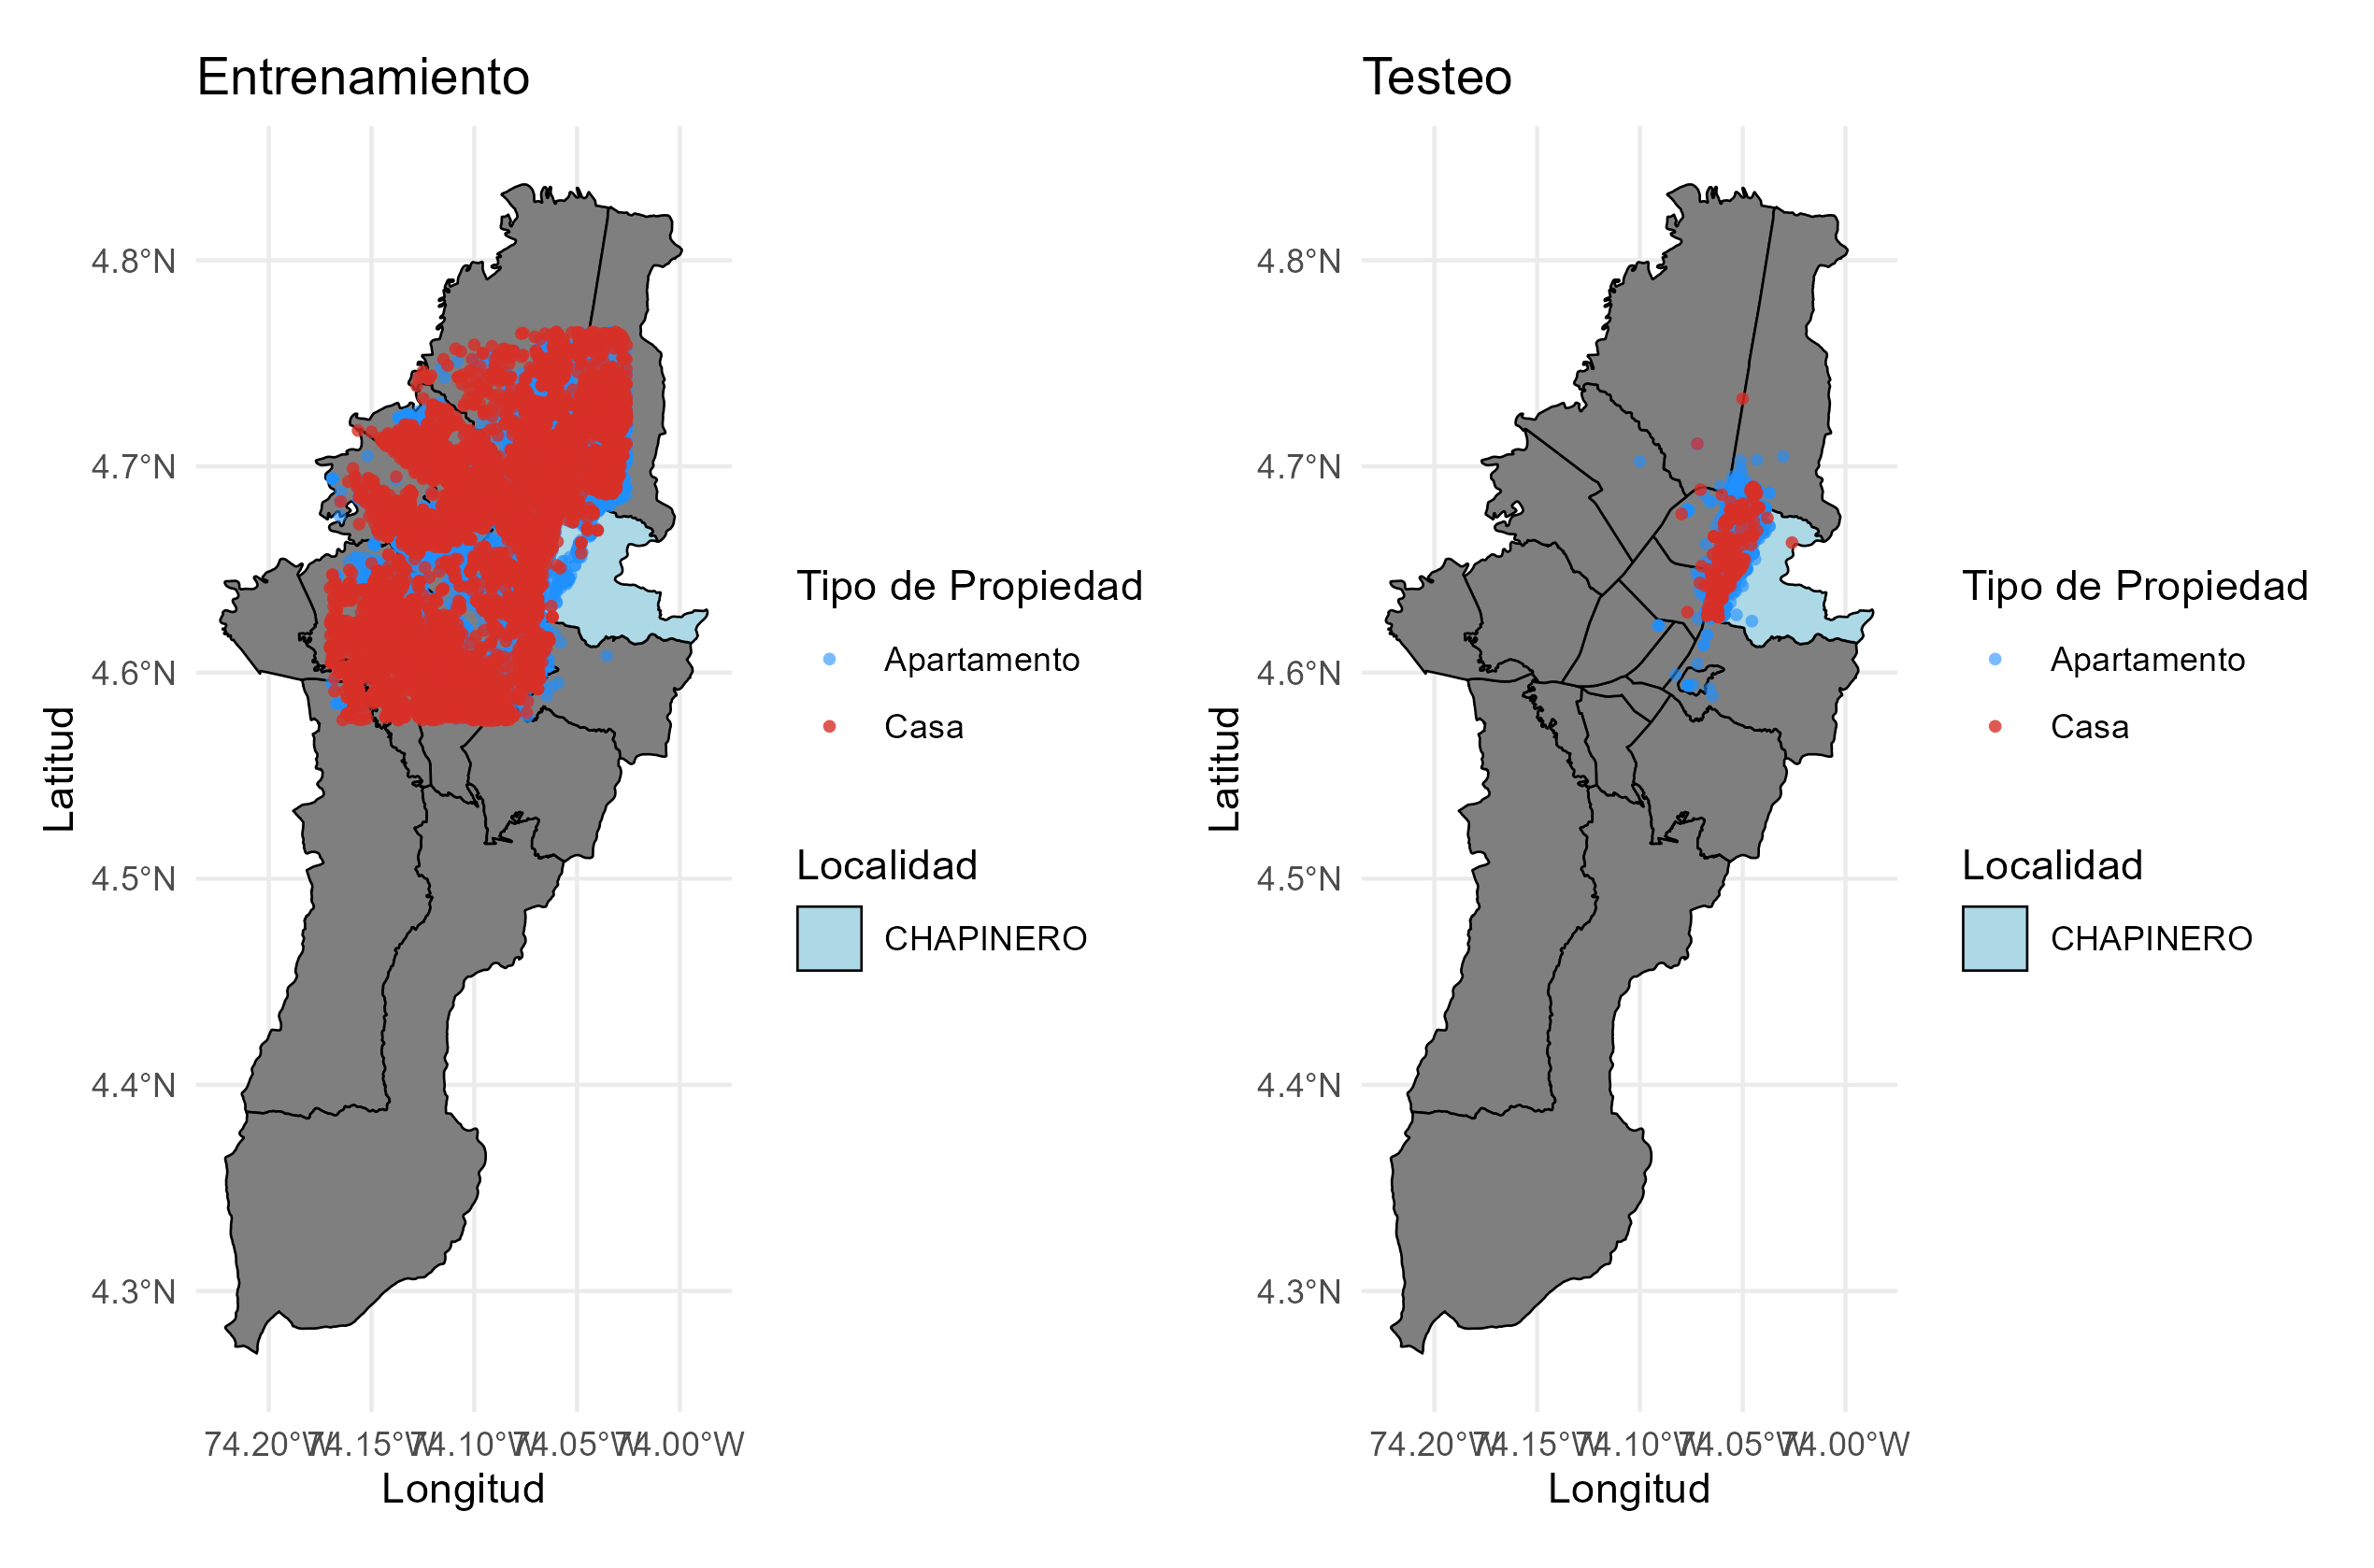
\includegraphics[width=0.55\linewidth]{Graficas/map_combined.png}
\end{figure}

Por el lado de la base de testeo, el 81,9\% de los datos sobre el área total de las propiedades y el 72,5\% de los valores correspondientes al área cubierta están ausentes. Asimismo, el 44,5\% de las observaciones carecen de información sobre el número de habitaciones, y el 24,2\% no contienen datos sobre el número de baños. Por otro lado, variables descriptivas como los títulos y las descripciones de los inmuebles, mantienen porcentajes mínimos de valores faltantes, con 0.0583\% y 0.0194\% respectivamente (Ver Anexo 1 - Figura 6). Esto evidencia la consistencia en los patrones de datos ausentes entre las bases y refuerza la necesidad de implementar estrategias de imputación adecuada.\\

\textbf{2.2 Limpieza de datos y selección de variables} \\

El tratamiento inicial de valores faltantes se realizó en varias etapas sobre ambas bases, implementando técnicas de imputación específicas según el tipo de variable  para asegurar la consistencia y calidad de los datos en análisis posteriores. Para las variables como baños y habitaciones, se aplicó la imputación por moda, reemplazando los valores ausentes con el valor más frecuente en cada categoría de vivienda. En el caso de las variables relacionadas con el área total y el área cubierta, se utilizaron dos enfoques: imputación por medias e imputación por mediana. La primera consistió en sustituir los valores faltantes con el promedio de los datos disponibles, mientras que la segunda utilizó el valor central de la distribución, mostrando mayor efectividad en presencia de datos sesgados o valores atípicos.\\

\textbf{Variables adicionales espaciales} \\

Se incorporan variables espaciales y textuales al análisis con el objetivo de enriquecer la comprensión de los factores que influyen en los precios de las propiedades, considerando tanto las características intrínsecas de las viviendas como su contexto urbano.De \href{https://www.openstreetmap.org/#map=6/4.63/-74.30}{Open Street Map (OSM)}, se obtuvieron diversas variables que reflejan las características del entorno urbano y que tienen un impacto directo en los precios de las propiedades. Estas variables incluyen:\\



\begin{multicols}{2}
\begin{itemize}[leftmargin=*]
    \item \textbf{Proximidad a parques:} Captura la distancia de cada propiedad al parque más cercano, considerando que la cercanía a áreas verdes aumenta la percepción de calidad de vida y bienestar.
    \item \textbf{Proximidad a estaciones de transporte público:} Registra la distancia a paraderos de buses o estaciones de transporte masivo, ya que la accesibilidad al transporte público es un factor determinante en la conectividad urbana.
    \item \textbf{Proximidad a centros comerciales:} Mide la distancia a los principales centros comerciales, que representan un acceso directo a servicios de consumo, entretenimiento y ocio.
    \item \textbf{Proximidad a hospitales:} Refleja la distancia al hospital más cercano, un aspecto importante para la seguridad y el acceso a servicios de salud.
    \item \textbf{Proximidad a colegios:} Indica la distancia a colegios o instituciones educativas de nivel básico y medio, un factor esencial para familias con hijos en edad escolar.
    \item \textbf{Proximidad a universidades:} Considera la distancia a instituciones de educación superior, lo que es relevante en zonas con alta población estudiantil o demanda de vivienda temporal.
    \item \textbf{Proximidad a supermercados:} Evalúa la distancia al supermercado más cercano, un indicador clave para medir la conveniencia y accesibilidad a servicios básicos.
    \item \textbf{Proximidad a avenidas principales:} Mide la distancia a las principales vías de la ciudad, reflejando el nivel de conectividad vehicular y acceso a transporte.
    \item \textbf{Proximidad a bares y restaurantes:} Incluye la distancia a establecimientos de ocio y gastronomía, lo que es un indicador del dinamismo social y cultural del área.
    \item \textbf{Proximidad a librerías y bibliotecas:} Analiza la cercanía a espacios culturales y educativos, considerados positivos para la percepción del entorno urbano.
    \item \textbf{Proximidad a gimnasios:} Mide la distancia a centros deportivos o gimnasios, reflejando el acceso a infraestructura para el bienestar físico.
    \item \textbf{Proximidad a bancos:} Considera la distancia a entidades financieras, especialmente relevante en zonas comerciales o de negocios.
\end{itemize}
\end{multicols}




De \href{https://www.ideca.gov.co/}{Infraestructura de Datos Espaciales de Bogotá (Ideca)}, se incorporaron capas de información relacionadas con los límites administrativos de localidades y barrios de Bogotá. Estas variables permiten clasificar las propiedades según su ubicación territorial, lo cual permite capturar las dinámicas espaciales que afectan los precios inmobiliarios. Las localidades y barrios actúan como proxies de factores territoriales, como infraestructura urbana, políticas de desarrollo, y características demográficas y socioeconómicas que pueden influir significativamente en la percepción de valor de las propiedades. Además, esta segmentación geográfica facilita el análisis de diferencias espaciales y patrones específicos dentro del mercado inmobiliario.\\

Por su parte, de la plataforma \href{https://datosabiertos.bogota.gov.co/} {Datos Abiertos de Bogotá}, se obtuvo información sobre el estrato socioeconómico de las propiedades. El estrato socioeconómico es un indicador relevante en Bogotá, ya que refleja el nivel de acceso a servicios básicos, la calidad de la infraestructura y el poder adquisitivo predominante en la zona. Incorporar esta información en el análisis permite modelar cómo las diferencias socioeconómicas impactan la valoración de las propiedades, siendo especialmente útil en un mercado con marcadas desigualdades. Cabe mencionar que, durante el proceso de integración de esta variable, se encontraron valores faltantes en algunas propiedades al intentar asignar el estrato socioeconómico. Para resolver esta situación, se realizó una imputación utilizando la moda del estrato con respecto a la localidad. \\

Estas variables no solo enriquecen el análisis al capturar elementos clave del entorno, sino que también permiten modelar con mayor precisión cómo los atributos externos influyen en la valoración de las propiedades. La inclusión de estos datos asegura un enfoque integral, donde se combinan las características intrínsecas de las viviendas con factores contextuales y urbanos.\\

\textbf{Variables adicionales de texto} \\

Adicionalmente, se generaron variables específicas a partir de las descripciones textuales de las propiedades, obteniendo información sobre características estructurales como el número de pisos en las casas o el piso donde se ubican los apartamentos. También se identificaron otras características, como la presencia de depósito, gimnasio, zona BBQ, parqueadero, entre otros. Para ello, se emplearon técnicas de normalización de texto, incluyendo la eliminación de caracteres especiales, la conversión a minúsculas y la extracción de información mediante patrones regulares.\\

\textbf{2.3 Estadística descriptiva}\\

La tabla de estadísticas descriptivas, la cual se puede observar a detalle en la sección de anexos, proporciona información clave para el análisis y predicción de precios de las propiedades. El precio promedio de las propiedades es de \$654.534.675, con una alta variabilidad reflejada en una desviación estándar de \$311.417.887. Los precios oscilan entre \$300.000.000 y \$1.650.000.000, indicando una amplia diversidad en el mercado inmobiliario que abarca desde propiedades accesibles hasta propiedades de lujo. El precio por metro cuadrado tiene un promedio de \$5,65 millones, con un máximo de \$40,45 millones, lo que evidencia una influencia significativa de la ubicación y el nivel socioeconómico.\\

Con relación a los precios, también se observa que la variable estrato presenta un promedio de 4,5. Este indicador en el mercado de vivienda colombiano está relacionado con un sector de la población de un nivel de ingreso medio-alto que demanda una serie de servicios de alto valor y que a su vez busca viviendas amplias y con aspectos complementarios como ascensor, balcón, servicios de entretenimiento cercanos y habitaciones adicionales. En cuanto a estas características estructurales, las propiedades tienen en promedio 3,1 dormitorios (rango: 0 a 11) y 2,7 baños (rango: 1 a 13), abarcando desde estudios pequeños hasta viviendas familiares grandes. La superficie total promedio es de 141.756 m², con valores entre 16 m² y 17,137 m², mientras que el área cubierta promedio es de 139.457 m², lo que sugiere diseños mayormente eficientes. Resalta, de igual forma, aspectos como la ubicación y la accesibilidad. En promedio, la distancia a un parque es de 159.030 m, al centro comercial de 234.067 m, a la avenida principal de 250.276 m y al transporte público de 944.568 m. Estos datos sugieren que muchas propiedades están estratégicamente ubicadas cerca de servicios recreativos y comerciales, así como de las principales vías de transporte, aunque estas últimas parecen estar más orientadas hacia el transporte privado. Dichas condiciones aumentan el valor percibido de las propiedades, ya que su precio no solo depende de sus características intrínsecas, sino también de factores externos asociados a su localización que podrían implicar una mayor valoración.\\

% ----- Correlación de las variables ----%
\textbf{2.4 Análisis de las variables}\\

% Disbtribucion de los precios en las propiedades
La Figura 2 muestra la distribución del precio de las propiedades, revelando una asimetría con sesgo positivo, donde la mayoría se concentra en rangos de precios bajos. El mayor número de propiedades (más de 4.000) se encuentra entre 200 y 400 millones de pesos, con un pico alrededor de los 400 millones. A medida que los precios aumentan, la cantidad de propiedades disminuye de forma progresiva, con una frecuencia significativamente menor en los rangos superiores a los 1.000 millones de pesos.  Este patrón sugiere un mercado inmobiliario enfocado en propiedades de menor costo, posiblemente reflejando las restricciones económicas y de financiación de los compradores promedio. Sin embargo, las propiedades de mayor valor, aunque menos frecuentes, representan un segmento exclusivo que puede ofrecer oportunidades estratégicas en mercados específicos.\\

Al analizar los precios por tipo de propiedad, la Figura 3 muestra cómo los apartamentos y las casas tienen distribuciones de precios distintas en el mercado inmobiliario. Los apartamentos presentan una clara concentración en el rango de 200 a 600 millones de pesos, lo que evidencia su accesibilidad para la mayoría de los compradores y su predominancia en la oferta del mercado. Por otro lado, las casas, aunque menos frecuentes, concentran su distribución en el rango de 300 a 800 millones de pesos, con precios promedio más altos que los de los apartamentos, lo que refleja su carácter más exclusivo.\\

Ambos tipos de propiedades muestran una disminución progresiva en frecuencia a medida que los precios aumentan, siendo poco comunes las viviendas que superan los 1,000 millones de pesos. Sin embargo, el mercado de apartamentos tiene una mayor cuota general, lo que refuerza su rol como la opción principal para la mayoría de los compradores, especialmente en Bogotá. El análisis de estas distribuciones evidencia que los apartamentos predominan en el mercado por su cantidad y accesibilidad económica, mientras que las casas, con un precio medio un 21\% superior al de los apartamentos en Bogotá, se destacan como una opción más exclusiva, dirigida a compradores con mayor capacidad adquisitiva.



\begin{figure}[H]
    \centering
    \begin{minipage}[t]{0.5\textwidth}
        \centering
        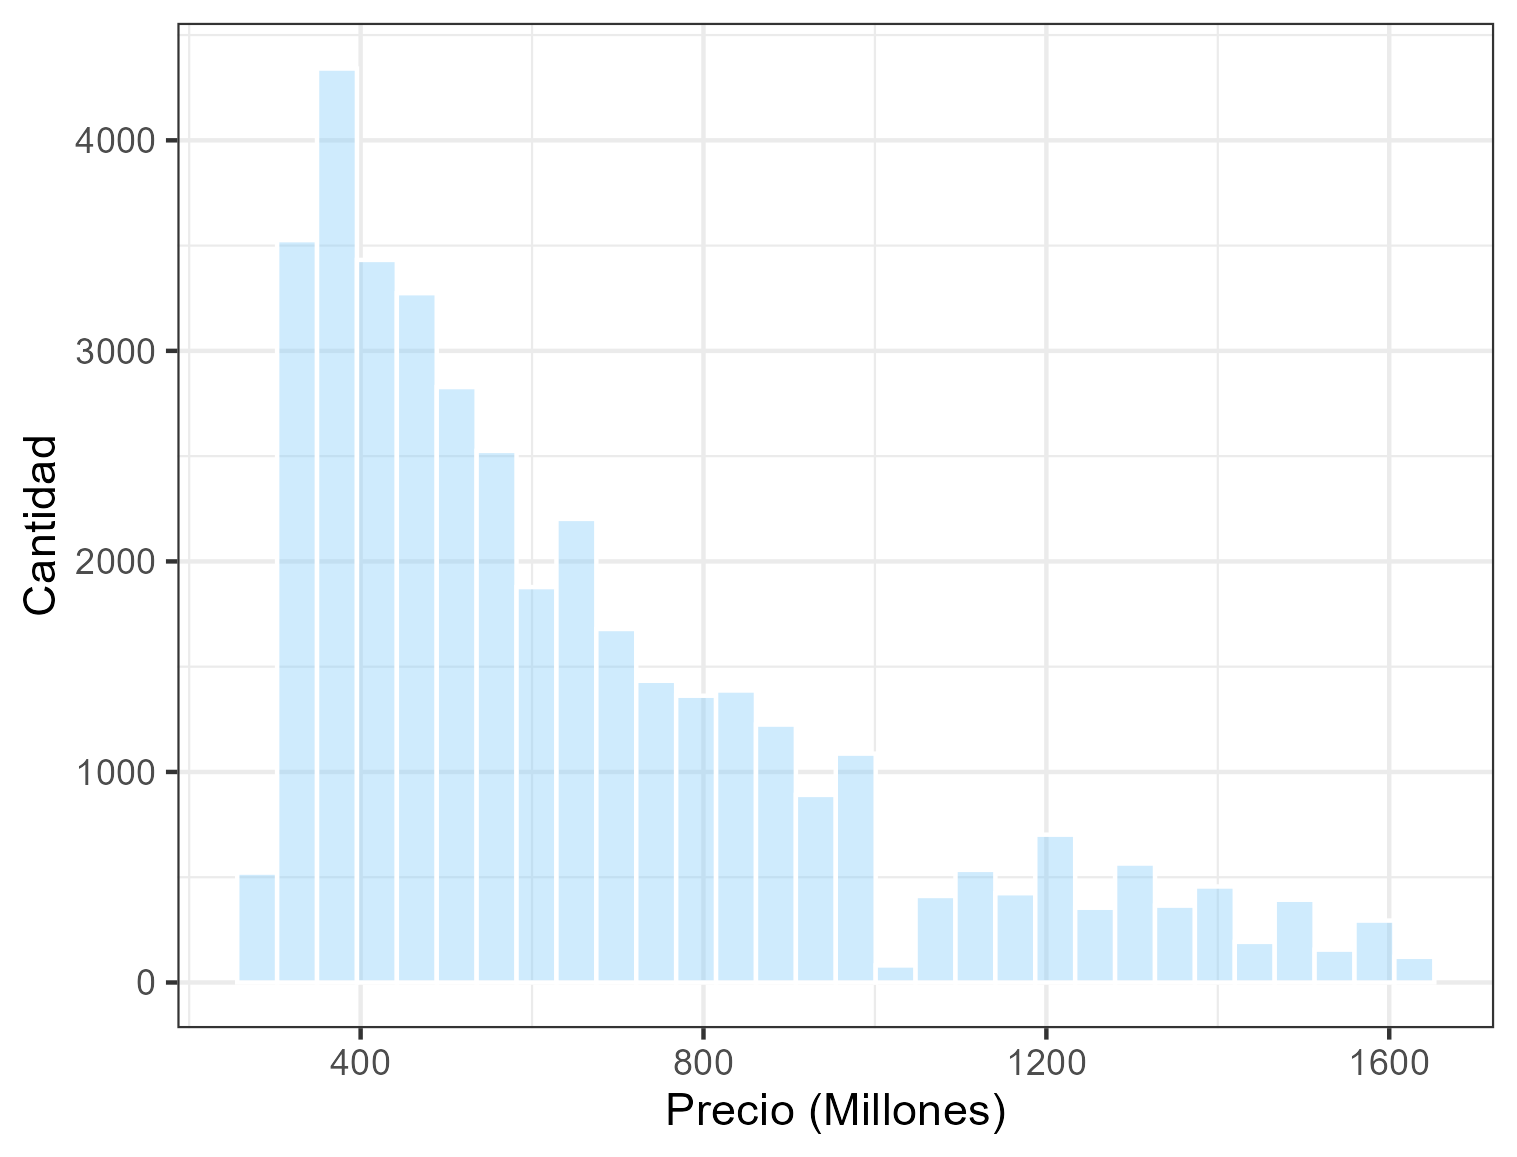
\includegraphics[width=\linewidth]{Graficas/Dis_precios2.png}
        \caption{Distribución del precio por tipo de propiedad}
    \end{minipage}%
    \hfill
    \begin{minipage}[t]{0.5\textwidth}
        \centering
        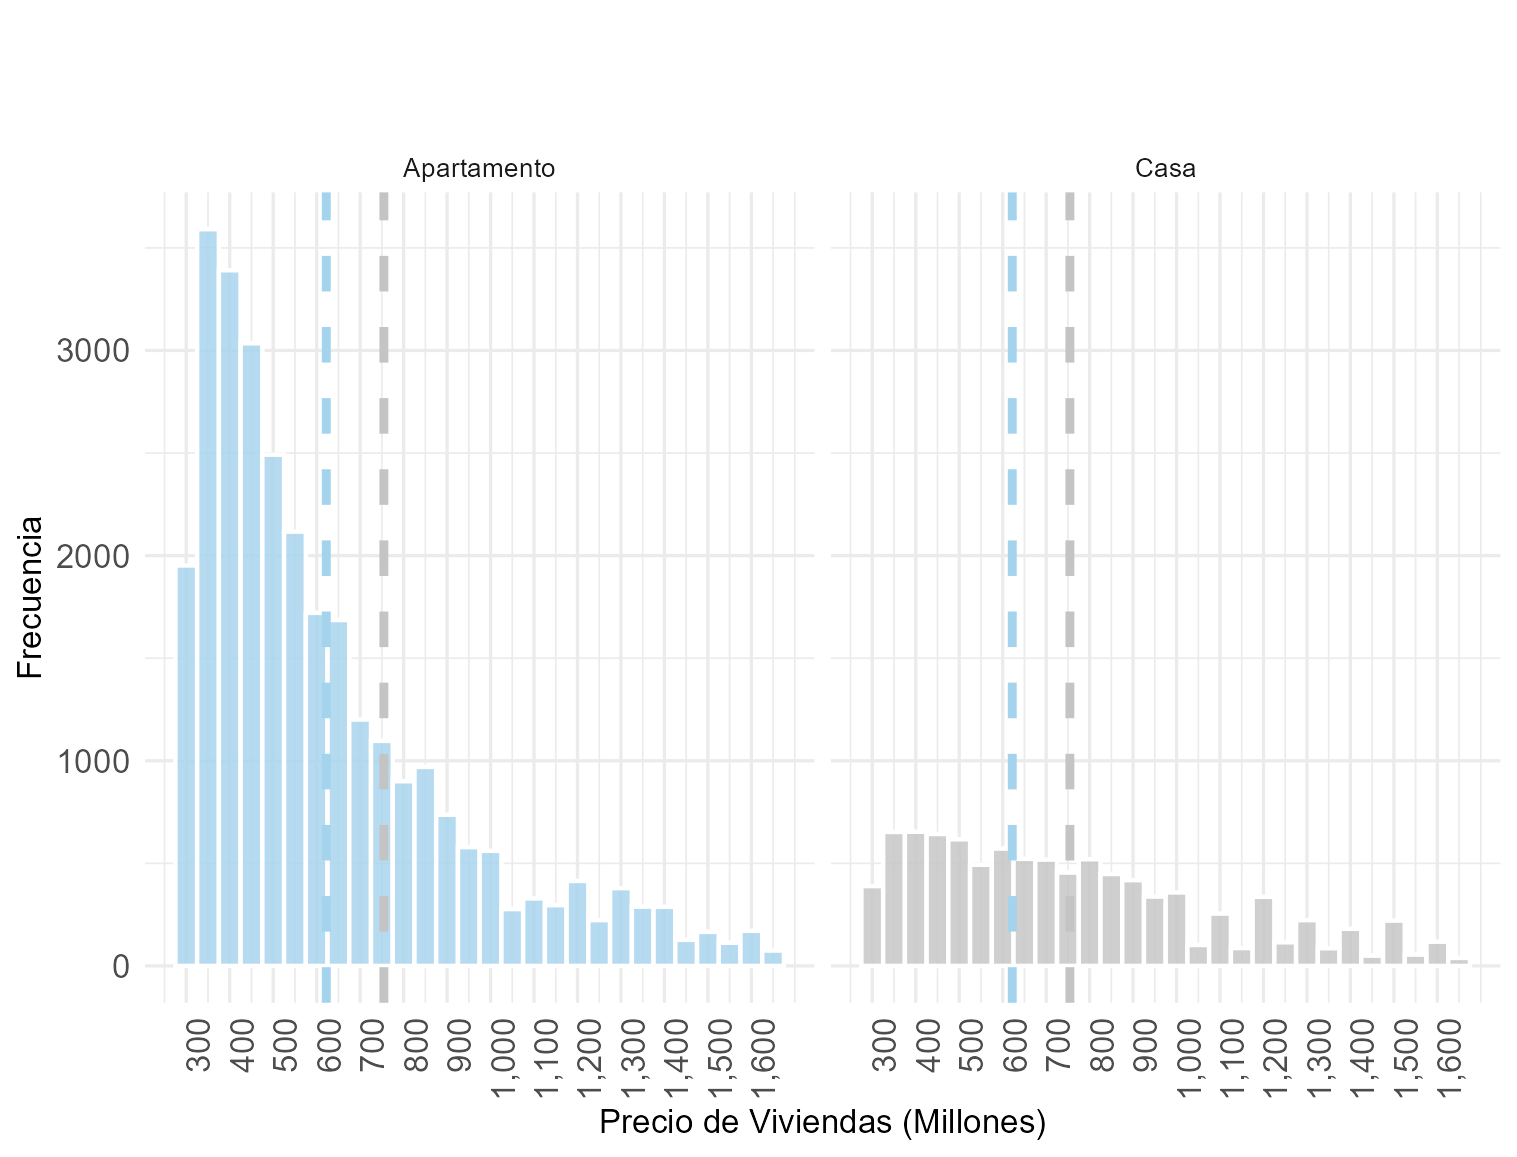
\includegraphics[width=\linewidth]{Graficas/Tipo_propiedad.png}
        \caption{Porcentaje de Apartamentos y Casas por Localidad}
    \end{minipage}
\end{figure}



Con respecto a la correlación entre variables, representada en el gráfico de correlación de las variables en los Anexos, muestra cómo diversas características internas y espaciales se relacionan con el precio de las propiedades. Los resultados indican que el número de baños imputados (Baños\_Imp) destaca con la correlación más alta (0,46), indicando que las propiedades con más baños tienden a ser más costosas, lo que subraya su relevancia en la valoración de inmuebles. La superficie cubierta imputada (Superficie\_Cubiert\_Imp) también presenta una correlación moderada de 0,32, evidenciando su impacto positivo en el precio. En contraste, la superficie total imputada (Superficie\_Total\_Imp) tiene una correlación menor de 0,14, lo que podría deberse a que no toda el área total tiene la misma utilidad o percepción de valor que el área cubierta.\\

Las variables relacionadas con la distancia a servicios, como estaciones de policía, gimnasios y supermercados, presentan correlaciones débiles con el precio de las propiedades. Entre estas, la distancia a la librería es la que más destaca, con una correlación de 0,24, aunque su influencia en el precio general sigue siendo baja. Sin embargo, aspectos como la cercanía a la avenida principal, parques y servicios de seguridad, aunque no muestran correlaciones significativas independientemente, tienen un valor relativo alto en la vida cotidiana, ya que impactan directamente en la accesibilidad, la calidad de vida, la tranquilidad y la percepción de seguridad de los residentes. Esto subraya la importancia de considerar estas variables en modelos más avanzados que integren su efecto combinado para una valoración más completa y precisa del precio de las propiedades.\\

Por último, la Figura 4 muestra la relación de apartamentos y casas por localidad. En localidades como Chapinero, Usaquén y Santa Fe, predomina una alta proporción de apartamentos, superando el 80 \% de las viviendas. Esto puede estar relacionado con las dinámicas urbanas de estas áreas centrales y de alta densidad poblacional, donde los apartamentos son más comunes debido a la optimización del espacio. Adicionalmente, según Cediel y Velásquez (2015), la ubicación estratégica de estas localidades, con fácil acceso a importantes avenidas, zonas comerciales y centros empresariales, las posiciona como focos de alta demanda para compradores que buscan calidad de vida y comodidad, lo cual repercute en el precio y concentra viviendas de lujo. Por otro lado, localidades como Barrios Unidos, Ciudad Bolívar y Suba presentan un mayor equilibrio o predominio de casas, lo que sugiere una oferta inmobiliaria más diversificada o centrada en vivienda unifamiliar, generalmente asociada a precios más asequibles en comparación con las zonas dominadas por apartamentos.

% Porcentaje de Apartamentos y Casas por Localidad
\begin{figure}[H]
    \centering
    \caption{Porcentaje de Apartamentos y Casas por Localidad}
    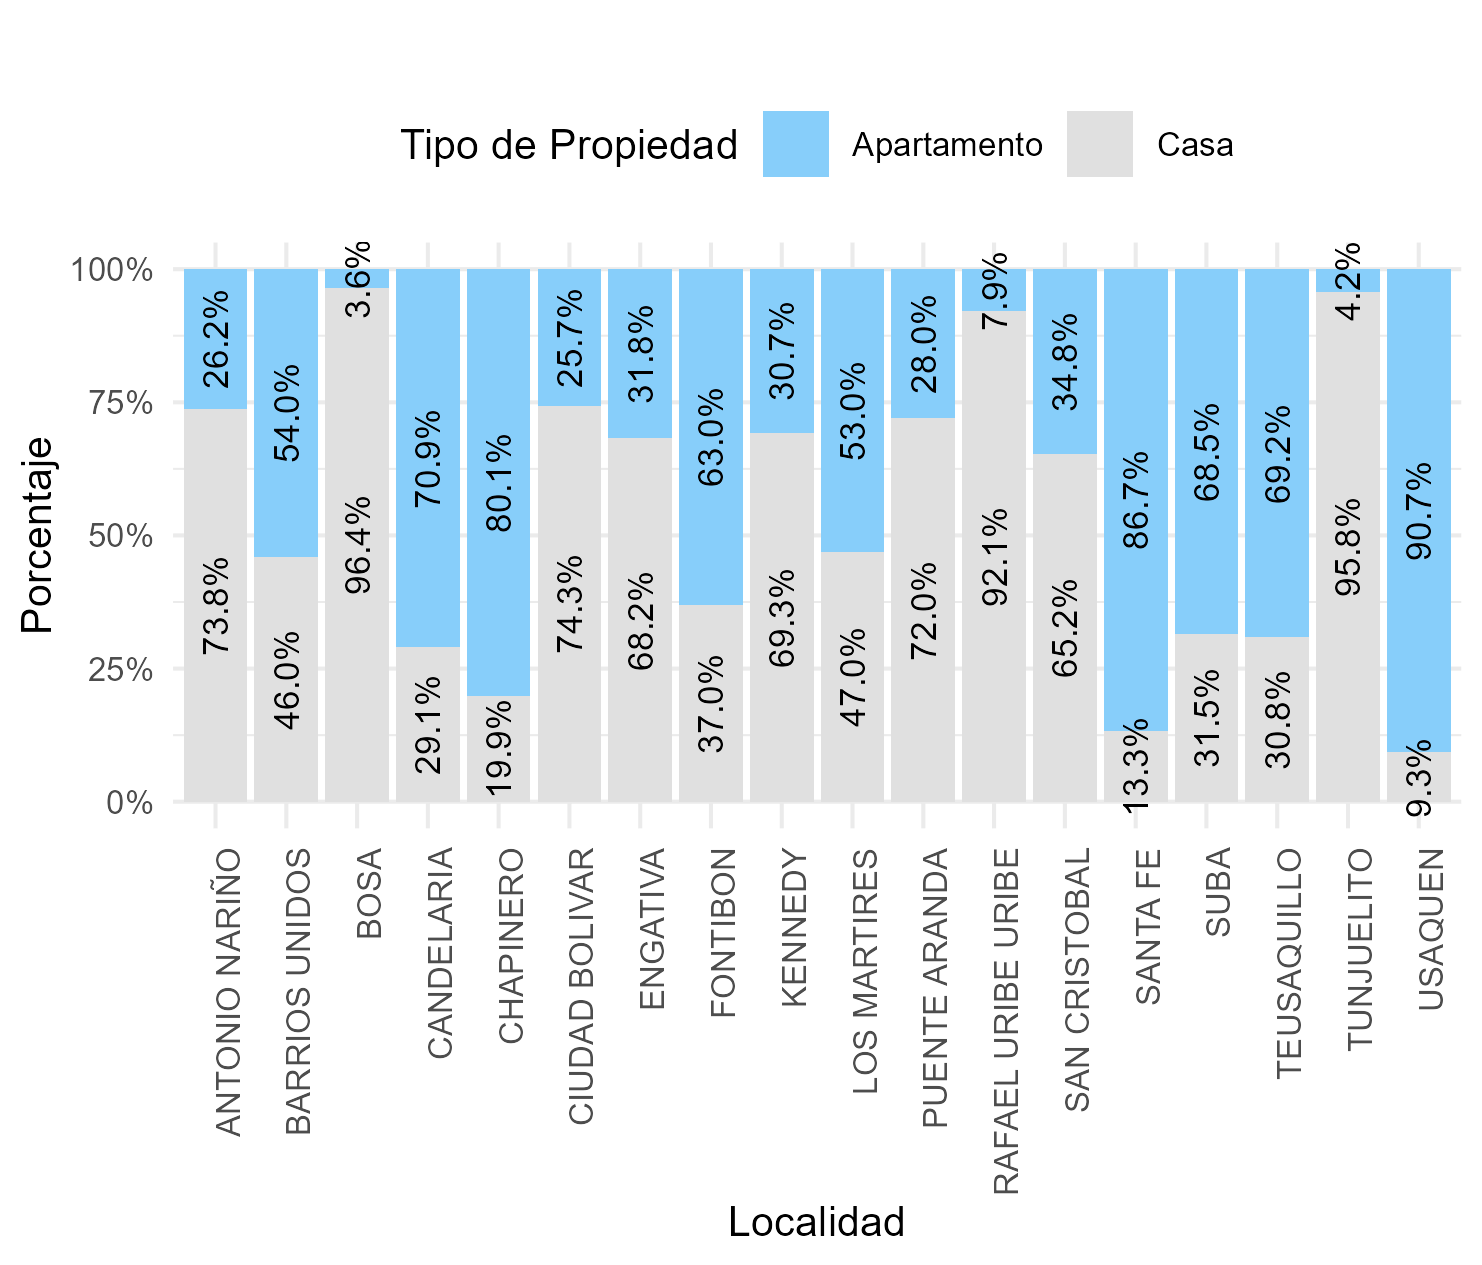
\includegraphics[width=0.4\linewidth]{Graficas/Tipo_propiedad_local.png}
\end{figure}

%-------------------------------------------------------%
\section{Modelos entrenados}

\subsection{Obtención de variables utilizadas}

Para entrenar los modelos, fue necesario incluir variables adicionales derivadas de las descripciones textuales de las propiedades en venta, así como variables espaciales deducidas a partir de su localización, las cuales fueron previamente descritas. Un aspecto clave del proceso fue el análisis y transformación de las descripciones de las propiedades. Para ello, se normalizó el texto, incluyendo  la conversión a minúsculas, la eliminación de caracteres especiales y puntuación, y la remoción de palabras irrelevantes o comunes (stopwords). La conversión anterior nos permitió construir una matriz termino-documento para observar la frecuencia de los términos de las descripciones.\\

Posteriormente, dada la cantidad de variables provenientes de esta matriz de texto, se aplicó análisis de componentes principales (PCA) para reducir su dimensionalidad. Esta técnica permitió condensar la información textual en un conjunto más pequeño de 72 componentes principales, capturando patrones clave en las descripciones y eliminando redundancias. Los componentes principales representaron de manera eficiente la variabilidad de los datos textuales, lo que facilitó su integración en los modelos predictivos.

\subsection{Random Forest y Superlearner} \\

Algunos de los modelos entrenados en este proceso fueron random forest, Elastic Net y la variante Ranger, esperando que cada uno capturara características que los demás no podían observar. El ensamblaje final combina las predicciones de estos modelos mediante el método NNLS (Non-Negative Least Squares), que asigna pesos no negativos a cada modelo para minimizar el error total. El Random Forest utilizado captura relaciones no lineales y efectos complejos entre las variables predictoras. Este modelo construye múltiples árboles de decisión independientes y utiliza sus promedios para predecir mediante una regresión. En este caso, se configuraron 1.000 árboles con diferentes valores de \textit{mtry} (número de variables evaluadas en cada división), logrando un balance entre diversidad y precisión. El Super Learner fue evaluado utilizando validación cruzada con 10 particiones (V=10), asegurando que los resultados reflejen la capacidad del ensamblaje para generalizar a nuevos datos.

\subsection{Regularización: Ridge y Elastic Net} \\

En este caso, se empleó validación cruzada espacial con cinco bloques (folds) representando cinco regiones espaciales distintas, validando los cálculos iterativamente en una de ellas para garantizar la robustez del modelo en un contexto inmobiliario, donde la ubicación tiene un impacto significativo en los precios. Adicionalmente, se implementaron dos recetas que incluyeron normalización, interacciones y transformaciones polinómicas, con el objetivo de capturar tanto relaciones lineales como no lineales, además de reducir la cantidad de variables utilizadas en el análisis. \\

El valor óptimo resultante, de \(\lambda = 0.0001\), indica una penalización baja, permitiendo que el modelo mantenga la mayoría de las variables. Esto es adecuado cuando las relaciones entre los predictores y la variable objetivo son complejas. Por otro lado, \(\alpha = 0.4\) combina la capacidad de \(L1\) para seleccionar variables relevantes y de \(L2\) para estabilizar los coeficientes frente a una alta correlación entre las variables utilizadas. En las variables predictoras utilizadas se destaca la distancia a servicios como parques, el transporte público, colegios, entre otros. Las variables utilizadas para este modelo se encuentran detalladas en el anexo de este documento. 

\subsection{Regresion Lineal}

El modelo ajustado de regresion lineal fue calculado con una transformación logarítmica del precio como variable dependiente (log(precio)). Esto estabiliza la varianza y mejora el ajuste en un rango amplio de valores de precios. La especificación del modelo incluye interacciones entre variables relevantes (distancia al parque, tipo de propiedad, etc.), términos polinómicos (grados 2 para distancia al parque y área del parque), y predictores tanto espaciales como estructurales y categóricos. Las variables utilizadas para este modelo se encuentran detalladas en el anexo de este documento.


\subsection{Redes neuronales}


El modelo de redes neuronales con mejor rendimiento utilizó tres capas ocultas, con 100, 50 y 10 nodos respectivamente, cada una con función de activación ReLU. Esta arquitectura capturó relaciones complejas y no lineales entre las variables predictoras y el precio de las propiedades, transformado logarítmicamente para estabilizar la varianza y mejorar la predicción de valores extremos. Aunque la ausencia de regularización mediante \textit{dropout} podría haber incrementado el riesgo de sobreajuste en un modelo con tantas capas y parámetros, este riesgo no se materializó. El uso de penalización y una tasa de aprendizaje controló la magnitud de los pesos, lo que permitió entrenar 8.471 parámetros y consolidó este modelo como el más eficiente entre los probados. Por otra parte, los 300 \textit{epochs} utilizados podrían haber incrementado el riesgo de sobreajuste si los datos fueran altamente ruidosos. Sin embargo, en este caso, la elección de este hiperparámetro dio como resultado una mejora significativa en las predicciones fuera de muestra con relación a los modelos con 200 \textit{epochs}. Las variables empleadas en este modelo se detallan en el anexo de este documento.







%-------------------------------------------------------%
\section{Resultados}

A continuación, se presenta una comparación de los resultados de todos los modelos utilizados en el proceso de predicción de los precios de la vivienda que fueron descritos en la sección anterior. Específicamente, la Tabla 1 muestra una comparación del desempeño fuera de muestra de acuerdo con la puntuación de Kaggle. 


\begin{table}[h]
\caption{Modelos de Predicción}
\vspace{3mm}
\centering
\resizebox{0.4\textwidth}{!}{ % Ajusta al ancho del texto
\begin{tabular}{c l r}
\toprule
\textbf{No. Modelo} & \textbf{Algoritmo}       & \textbf{Puntaje Kaggle}  \\ 
\midrule
1                   & Regresión Lineal        & 272.534.440                                   \\
2                   & Elastic Net             & 247.822.060                                       \\
3                   & Random Forest           & 253.324.887                                          \\
4                   & XGBoost                 & 227.441.318                                       \\
5                   & Redes Neuronales        & 235.656.787                                          \\
\bottomrule
\end{tabular}
}
\label{tab:modelos_prediccion}
\end{table}

\subsection{Modelo elegido: XGBoost}

El modelo con la mejor capacidad predictiva sobre el precio de la vivienda de acuerdo con la Tabla 2 se estimó usando el algoritmo de XGboost, donde la métrica MAE alcanzó un valor de 227.441.318 en Kaggle. Este algoritmo representó una mejora importante comparativamente a la segunda mejor predicción obtenida a través de Redes Neuronales. La forma funcional de este modelo se puede observar en los anexos, en la subsección de modelos. Estas variables fueron seleccionadas en la medida que permiten abordar 4 grandes factores relevantes que determinan el precio de las viviendas: \\

\textbf{1) Ciclo económico:} Las variables de mes y año capturan el ciclo de la economía nacional. En particular, en periodos de alto crecimiento económico, el precio de las viviendas suele elevarse y, por tanto, tener presente la fecha de anuncio de venta puede ayudar a capturar la estacionalidad de este tipo de precios.\\

\textbf{2) Tamaño y distribución:} Las variables referentes a las características estructurales de la vivienda, tales como el área total, el número de habitaciones, baños o pisos, son fundamentales en la valoración de los bienes raíces, pues es de esperarse que entre mayor sea el tamaño de la vivienda, mayor sea  su precio. En ese mismo sentido, se incluyó la proporción de baños, cuartos y dormitorios con respecto al área total, para identificar cómo se distribuye dicho tamaño. Adicionalmente, se incluyeron términos cuadráticos con el objetivo de capturar posibles no linealidades de dichas variables, tales como la menor influencia del número de baños después de cierto umbral. Por ejemplo, un baño es fundamental en un inmueble de 3 dormitorios, pero para este mismo número de dormitorios, un cuarto baño es menos indispensable. \\

\textbf{3) Ubicación:} Las variables del estrato, localidad y en general las variables de distancia a ciertos puntos de interés (parques, estaciones de transporte público, colegios, etc.) capturan el efecto del entorno socioeconómico y el acceso a servicios de los inmuebles, los cuales son fundamentales en las decisiones de compra de los demandantes, y por consiguiente, en su proceso de valoración. En particular, propiedades con características de tamaño y distribución similares pueden tener un precio diferente por su ubicación distinta y, por tanto, por su acceso diferenciado a servicios de la vida cotidiana. \\

\textbf{4) Características específicas:} Las variables de texto y los componentes principales obtenidas a partir del filtro de las descripciones de los anuncios de venta de las viviendas, se incluyeron en la medida que permiten capturar características propias de cada inmueble, cuya existencia o acceso pueden ser determinantes en el proceso de valoración. En particular, el servicio de GYM o la existencia de elevador, puede ser un diferencial fundamental en el proceso de compra, incluso si se tratase de inmuebles con tamaño y ubicación similares.  \\

Para su estimación primero se dividió de forma aleatoria la muestra de prueba original conservando el 80\% de las observaciones. Esto se hizo con el objetivo de contar con una muestra de testeo propia (correspondiente al 20\% de la muestra de prueba original) para evaluar entre los distintos modelos el que mejor se comportaba fuera de muestra antes de subir el resultado a Kaggle. Sobre dicha base de prueba se llevó a cabo además un proceso de validación cruzada espacial, y con base en esta, se seleccionaron los hiperparámetros que minimizaron el MAE. El proceso de validación cruzada espacial con 5 pliegues, fue fundamental para disminuir la dependencia de las observaciones por cuenta de  la auto-correlación espacial. En la figura 8 del Anexo se presenta la distribución de los datos en cada uno de los cinco pliegues indicados a través de diferentes colores. En la Tabla 2, se puede observar la grilla sobre la que se hizo la búsqueda de hiperparámetros y los que finalmente fueron seleccionados de acuerdo a este enfoque. Con los hiperparámetros seleccionados,  el modelo tuvo un MAE dentro de la muestra de 48.688.390. Al evaluarse sobre el conjunto de testeo propio, se obtuvo un MAE de 106,693,941. Finalmente, al evaluarse sobre el test de Kaggle, el MAE obtenido fue 227.441.318. 


\begin{table}[h!]
\centering
\caption{Hiperparámetros evaluados y seleccionados para XGBoost}
\label{tab:hiperparametros}
\resizebox{0.6\textwidth}{!}{ % Ajusta el ancho relativo
\begin{tabular}{l|c|c}
\hline
\textbf{Parámetros} & \textbf{Evaluados} & \textbf{Seleccionado} \\ \hline
Número de árboles (nrounds) & 300; 500 & 500 \\ \hline
Profundidad máxima (max\_depth) & 4; 6 & 6 \\ \hline
Tasa de aprendizaje (eta) & 0.01; 0.05; 0.1; 0.15 & 0.15 \\ \hline
Observaciones mínimas por hoja (min\_child\_weight) & 10; 20; 30 & 10 \\ \hline
Parámetro de regularización (gamma) & 0; 0.1; 0.15; 0.2 & 0.15 \\ \hline
Proporción de predictores (colsample\_bytree) & 0.33; 0.66 & 0.66 \\ \hline
Fracción de datos (subsample) & 0.4; 0.8 & 0.8 \\ \hline
\end{tabular}
}
\vspace{0.5mm}

\scriptsize
\textbf{Nota:} Entre paréntesis se muestra la identificación del hiperparámetro en el lenguaje de programación de R.
\end{table}

La variable más importante en la estimación fue la razón entre el número de baños y el área total del inmueble. Este resultado sugiere que la distribución de la propiedad en términos de disponibilidad de baños, es un buen predictor de los precios de las viviendas de Bogotá. Esta conclusión se confirma también con la buena capacidad predictora de la razón entre dormitorios y el área total del inmueble, la cual se ubicó como la tercera variable más relevante. Por su parte, la variable de estrato fue la segunda más relevante. Esta, junto con las variables de distancia del inmueble a la librereria y a la estación más cercana del bus, que fueron respectivamente la cuarta y quinta más relevante, dan cuenta que la ubicación socioeconómica en la ciudad, así como el acceso a ciertos servicios para el desarrollo normal de la vida cotidiana, son factores fundamentales en el proceso de valoración de la vivienda. 

\section{Conclusiones}

En el presente documento se llevó a cabo un análisis detallado de los precios de la vivienda en Bogotá, con el objetivo de construir un modelo predictivo de los precios de la vivienda de la localidad de Chapinero. Para ello, se identificaron un conjunto de predictores que abordan las características estructurales de la vivienda tales como el tamaño o la distribución de las alcobas, variables geográficas que permiten ubicar la vivienda en relación con ciertos puntos de interés como parques, estaciones de transporte público, entre otras, así como variables con características específicas de cada vivienda obtenidas a través de la descripción textual de la vivienda. \\

A través de la aplicación de diversos algoritmos de regresión de machine learning, se buscó el mejor modelo predictivo de los precios. De todos los modelos entrenados, el construido a través del algoritmo de XGBoost fue el que presentó el mejor rendimiento en términos predictivos de acuerdo con la MAE, alcanzando un valor de 227,441,318. La precisión del modelo XGBoost en este contexto puede explicarse por su capacidad de manejar grandes volúmenes de datos y captar relaciones no lineales entre variables. Las variables más influyentes en el modelo, calibrado usando un proceso de validación cruzada espacial, fueron en primera instancia las referentes a organización de la propiedad (a través de la razón entre el número de baños y el área total del inmueble y la razón entre el número de dormitorios y el área total del inmueble) y en segunda instancia, aquellas referentes a las características socioeconómicas y de ubicación (estrato y distancia a librería y estación más cercana del bus).  Se destaca que el segundo modelo con mejores resultados correspondió al calibrado con redes neuronales. De esta manera, los mejores modelos parecen ser aquellos que reconocen relaciones complejas entre las variables predictoras. De esta forma, para mejorar los resultados futuros, se recomienda por un lado seguir explorando este tipo de algoritmos, buscando sobre un conjunto más amplio de hiperparámetros, dadas las limitaciones computacionales del presente análisis. De esta forma, se podría mejorar el proceso de predicción y evitar pérdidas asociadas a un sobrevaloración de los inmuebles tal como sucedió con la empresa Zillow. 


\section{Referencias}

\begin{itemize}
    \item Cediel Sánchez, V. \& Velásquez Vega, C. (2015).
    \textit{ ¿Hay una burbuja inmobiliaria en Bogotá? Un estudio por segmentos de mercado}. Revista de Economía Institucional. 17, 32 (jun. 2015), 233–257.
    \item Chou, J. S., \& Truong, D. N. (2022). \textit{Comparison of machine learning models to provide preliminary forecasts of real estate prices}. \textit{Journal of Housing and the Built Environment}.
    \item Grajales Alzate, Y. V. (2019).\textit{Modelo de predicción de precios de viviendas en el Municipio de Rionegro para apoyar la toma de decisiones de compra y venta de propiedad raíz} (Master's thesis, Escuela de Ingenierías).
    \item García Camargo, P. A. (2021).\textit{Implementación de un modelo machine learning para la estimación del valor del metro cuadrado de un inmueble ubicado en Cundinamarca}. Universidad Nacional.
    \item Imbachi, F. J., \& Ramírez, A. A. (2023). \textit{Modelo de Machine Learning para la Estimación del Valor Comercial de un Inmueble en Neiva}. Universidad Surcolombiana.
    \item Nieto, M. A. (2022). \textit{Modelo de Aprendizaje Automático para la Predicción de Precios de Vivienda en la Ciudad de Bogotá}. Apuntes de Ciencia e Ingeniería.
    \item Rosen, S. (1974). \textit{Hedonic Prices and Implicit Markets: Product Differentiation in Pure Competition}. \textit{Journal of Political Economy}.
    \item Sicilia Gómez, B. (2024). \textit{Desarrollo de Modelos de Predicción de Precios Inmobiliarios Utilizando Técnicas de Machine Learning:Un Enfoque Comparativo}. Universidad Pontificia Comillas.
\end{itemize}





%-------------------------------------------------------%
\section{Anexos}

\subsection{Estadísticas Descriptivas}
\begin{table}[H]
    \centering
        \caption{Estadísticas descriptivas}
    \resizebox{\textwidth}{!}{%
        
\begin{tabular}{@{}lccccc@{}}
\toprule
\textbf{Variable}                    & \textbf{N}      & \textbf{Media}     & \textbf{Desv. Est.} & \textbf{Mínimo}   & \textbf{Máximo}      \\ \midrule
Precio                          & 38,644 & 654,534,675.000 & 311,417,887.000 & 300,000,000 & 1,650,000,000 \\
Precio por m2                   & 38,644 & 5.648           & 2.792           & 0.020       & 40.450       \\
Mes                             & 38,644 & 5.665           & 3.289           & 1           & 12           \\
Año                             & 38,644 & 2,020.294       & 0.760           & 2,019       & 2,021        \\
Dormitorios                     & 38,644 & 3.145           & 1.535           & 0           & 11           \\
Latitud                         & 38,644 & 4.691           & 0.037           & 4.577       & 4.765        \\
Longitud                        & 38,644 & -74.063         & 0.032           & -74.170     & -74.026      \\
Habitaciones (Imp.)             & 38,644 & 3.149           & 1.056           & 1           & 11           \\
Baños (Imp.)                    & 38,644 & 2.704           & 1.008           & 1           & 13           \\
Superficie Total (Media Imp.)   & 38,644 & 141.756         & 131.934         & 16.000      & 17,137.000   \\
Superficie Cubierta (Media Imp.)& 38,644 & 139.457         & 58.461          & 2.000       & 1,336.000    \\
Superficie Total (Mediana Imp.) & 38,644 & 127.227         & 130.006         & 16          & 17,137       \\
Superficie Cubierta (Mediana Imp.) & 38,644 & 131.082      & 59.252          & 2           & 1,336        \\
Habitaciones (Imp. 2)           & 38,644 & 3.109           & 1.042           & 1           & 11           \\
Baños (Imp. 2)                  & 38,644 & 2.696           & 1.010           & 1           & 13           \\
Superficie Total (Media Imp. 2) & 38,644 & 149.393         & 127.616         & 16.000      & 17,137.000   \\
Superficie Cubierta (Media Imp. 2) & 38,644 & 135.526      & 51.025          & 2.000       & 1,336.000    \\
Superficie Total (Mediana Imp. 2) & 38,644 & 127.222       & 128.380         & 16          & 17,137       \\
Superficie Cubierta (Mediana Imp. 2) & 38,644 & 124.349    & 53.478          & 2.000       & 1,336.000    \\
Número de Pisos (Casa)      & 38,644 & 1.082           & 0.442           & 1           & 10           \\
Piso (Apartamento)                 & 38,644 & 2.396           & 2.218           & 1           & 34           \\
Distancia al Parque             & 38,644 & 159.030         & 99.981          & 0.991       & 3,344.620    \\
Área del Parque                 & 38,644 & 6,979.706       & 25,240.860      & 20.056      & 975,008.400  \\
Distancia a la Policía          & 38,644 & 1,016.765       & 510.055         & 2.416       & 2,957.094    \\
Distancia al Gimnasio           & 38,644 & 899.716         & 650.906         & 6.297       & 4,959.468    \\
Distancia al Transporte Público & 38,644 & 944.568         & 654.997         & 4.023       & 3,834.865    \\
Distancia al Supermercado       & 38,644 & 410.284         & 258.707         & 2.052       & 3,647.074    \\
Distancia al Bar                & 38,644 & 1,382.015       & 699.443         & 4.663       & 3,968.576    \\
Distancia al Hospital           & 38,644 & 923.326         & 534.796         & 9.743       & 3,565.820    \\
Distancia al Colegio            & 38,644 & 536.494         & 299.135         & 4.862       & 1,725.529    \\
Distancia al Centro Comercial   & 38,644 & 308.098         & 234.067         & 0.231       & 3,494.995    \\
Distancia al Restaurante        & 38,644 & 386.392         & 260.806         & 1.068       & 2,741.448    \\
Distancia a la Librería         & 38,644 & 2,446.302       & 1,140.723       & 13.801      & 4,624.506    \\
Distancia a la Universidad      & 38,644 & 1,066.883       & 569.696         & 3.194       & 4,338.044    \\
Distancia al Banco              & 38,644 & 675.310         & 510.746         & 3.498       & 4,724.606    \\
Distancia a la Avenida          & 38,644 & 276.898         & 250.276         & 0.000       & 1,974.753    \\
Estrato (Imp.)                  & 38,644 & 4.523           & 1.455           & 0           & 6           \\ \bottomrule
\end{tabular}%

    }
    \label{tabla_estadisticas}
    \begin{tablenotes}
        \footnotesize
        \item \textbf{Nota:} Las variables que tienen \textit{Imp.2} fueron imputadas utilizando la nueva variable de tipo de propiedad, lo que permitió completar valores faltantes con base en dicha característica.
    \end{tablenotes}
\end{table}


\subsection{Correlación de las variables}

% Correlación de las variables
\begin{figure}[H]
    \centering
    \caption{Correlación de las variables}
    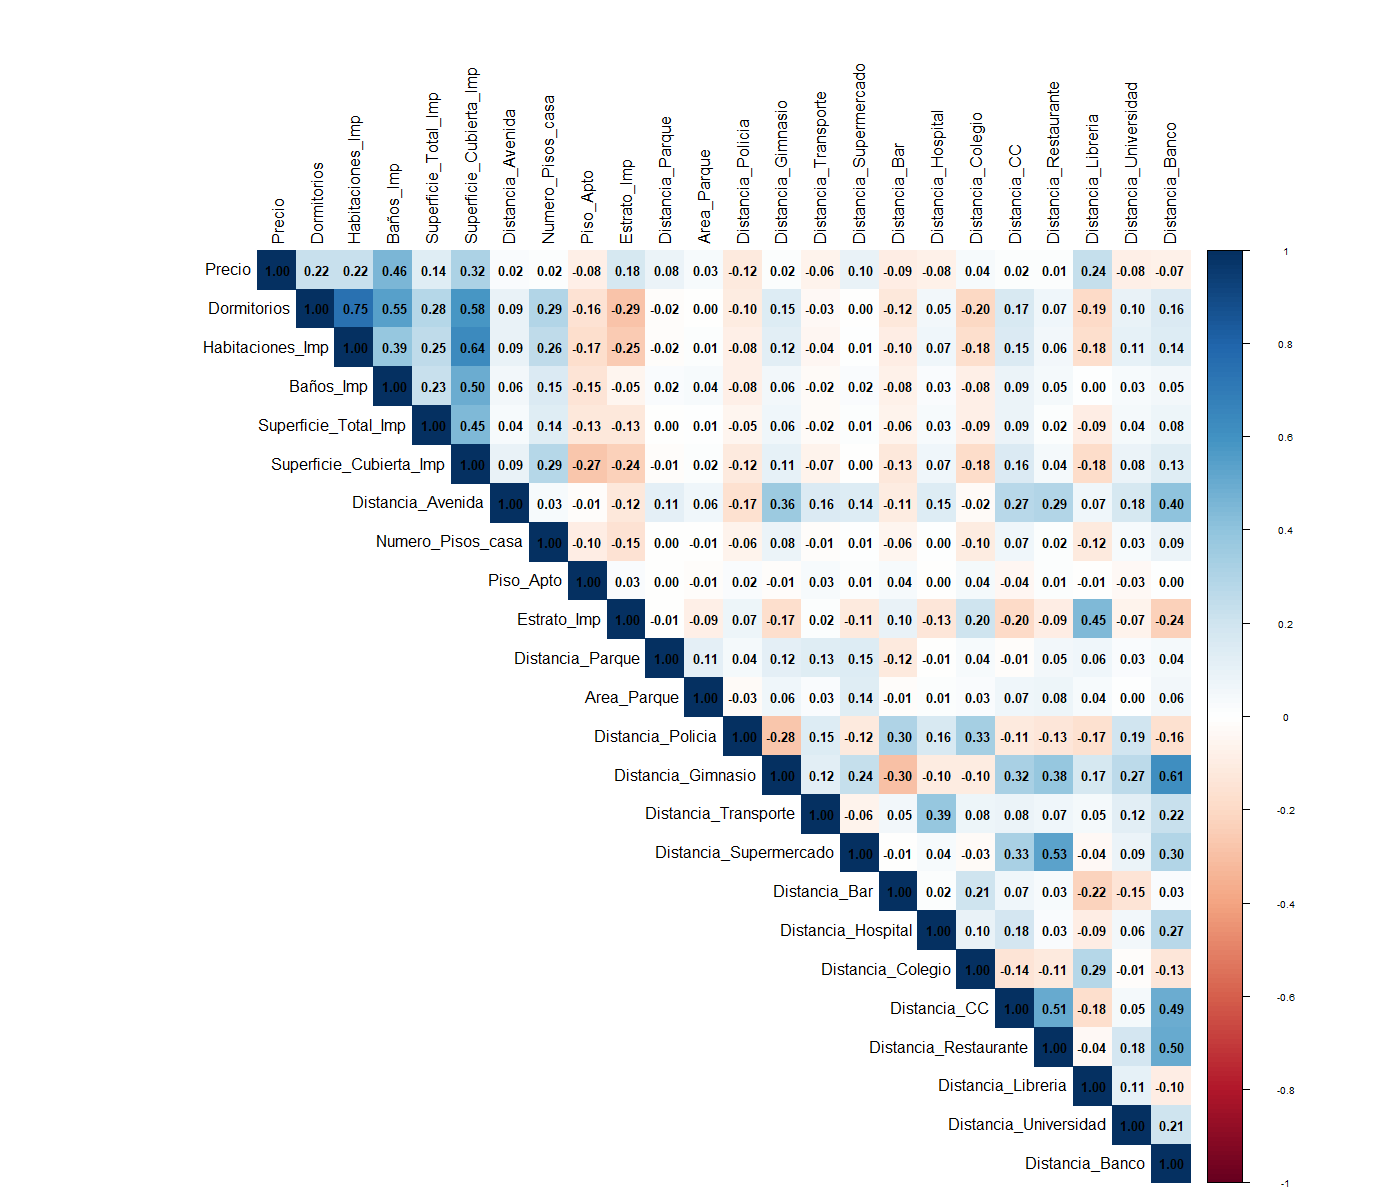
\includegraphics[width=0.9\linewidth]{Graficas/graf_corr_completa.png}
\end{figure}


%-------missings de la base-----%

\subsection{Missing values}
\begin{figure}[H]
    \centering
    \caption{Valores faltantes de las variables de la base testeo}
    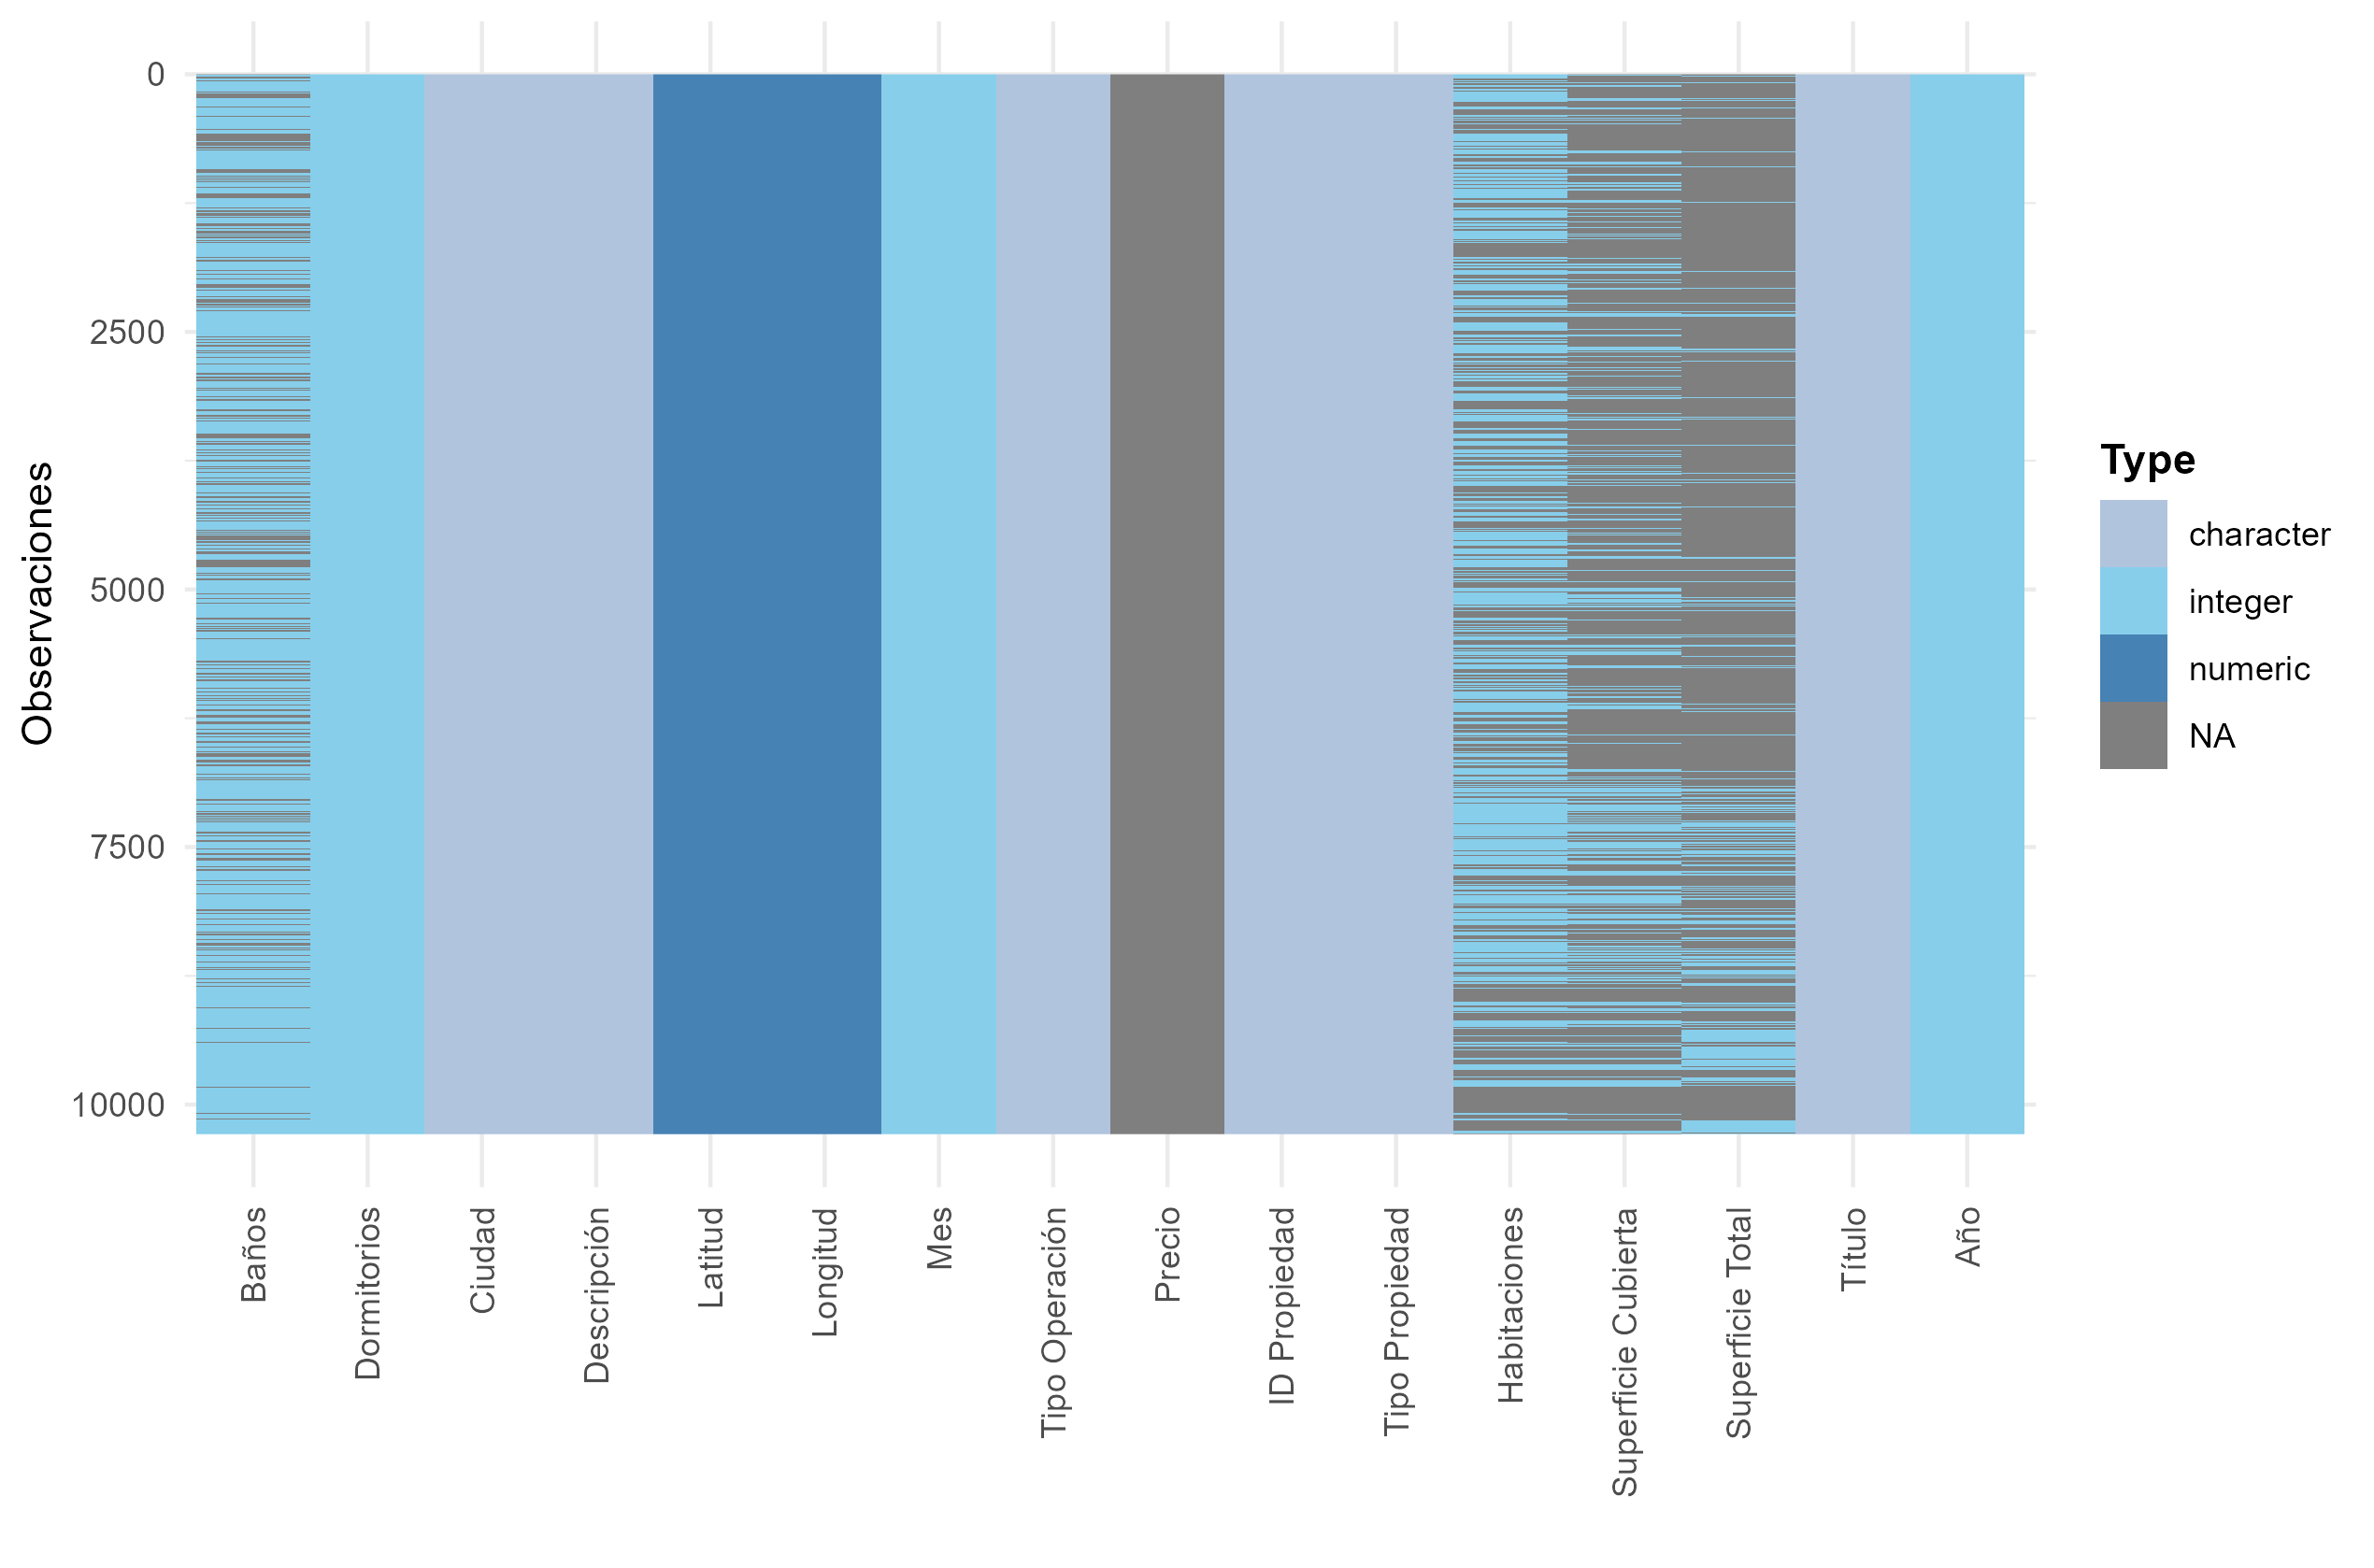
\includegraphics[width=0.75\linewidth]{Graficas/graf_miss_f2_test.png}
\end{figure}

%-----  Missings de las bases ------------%
\begin{figure}[H]
    \centering
    \caption{Valores faltantes de las variables de la base Entrenamiento }
    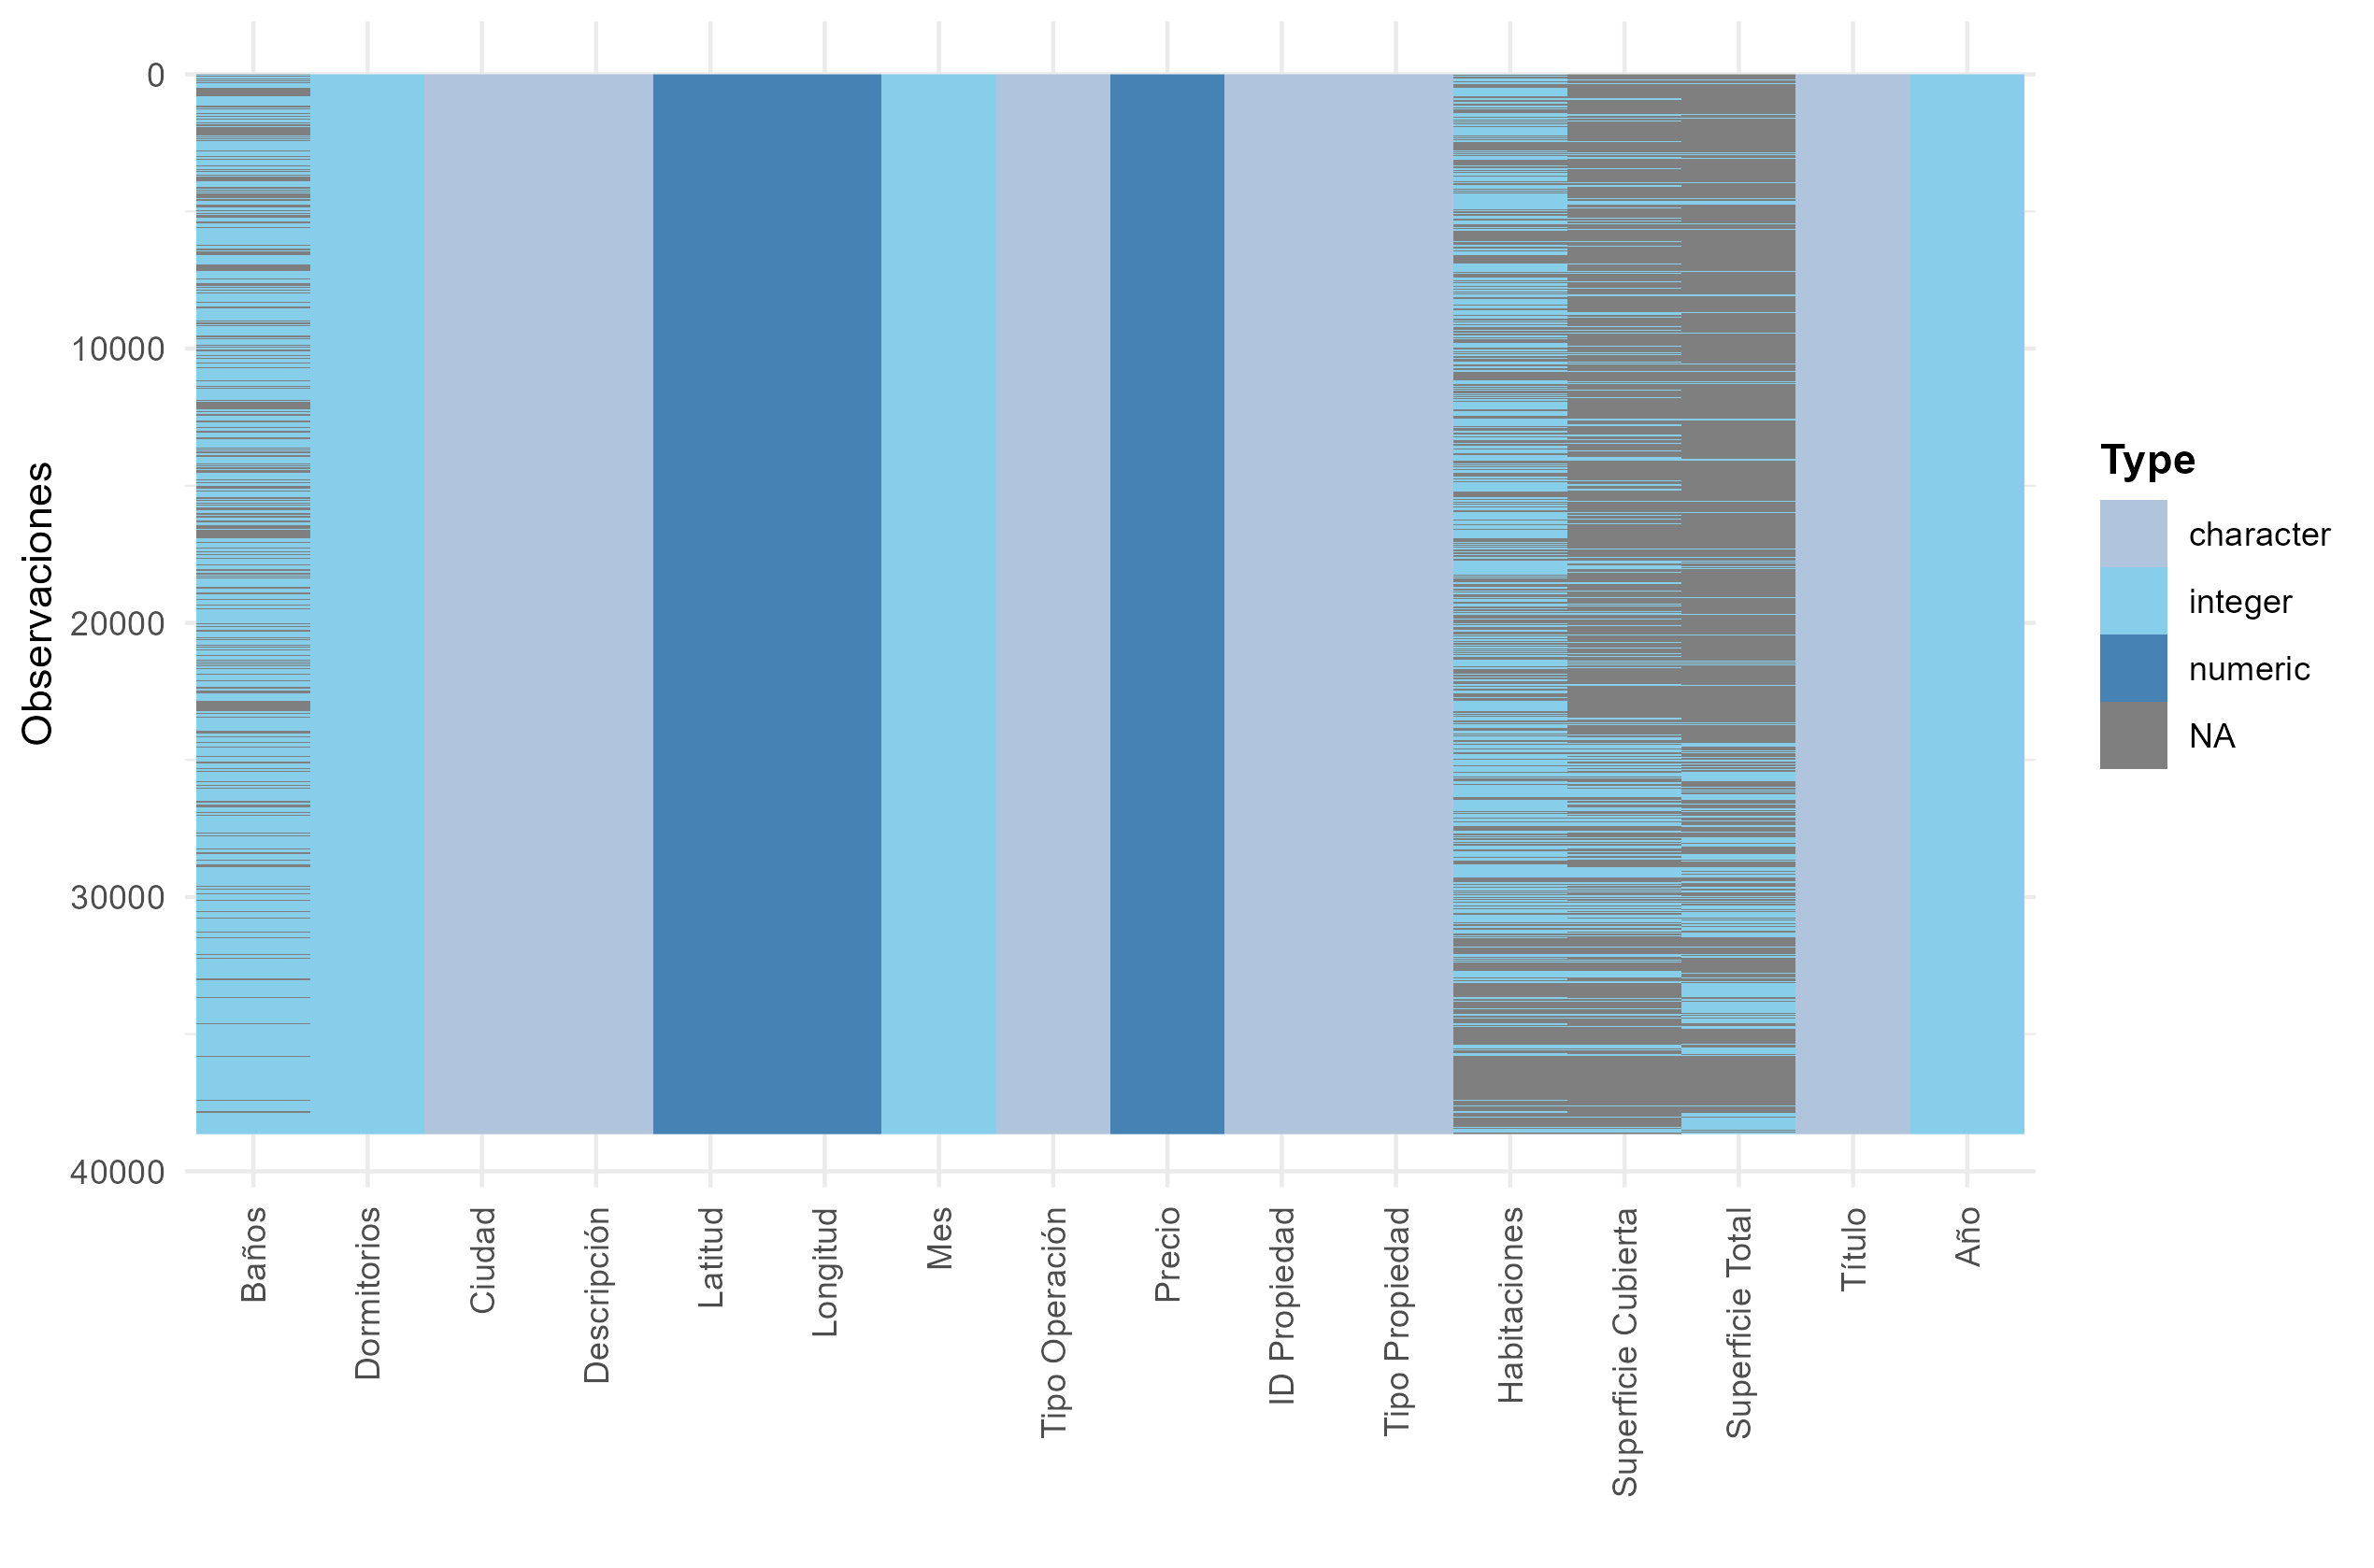
\includegraphics[width=0.75\linewidth]{Graficas/graf_miss_f2_train.png}
\end{figure}


\subsection{Modelos}

\subsubsection{Variables utilizadas en modelo de Boosting}

\begin{table}[h!]
\centering
\begin{tabular}{l|p{12cm}}
\hline
\textbf{Categoría} & \textbf{Variables} \\ \hline
\textbf{Variables espaciales} & Distancia al parque, Área del parque, Distancia a la policía, Distancia al gimnasio, Distancia al transporte público, Distancia al supermercado, Distancia al bar, Distancia al hospital, Distancia al colegio, Distancia al centro comercial, Distancia al restaurante, Distancia a la librería, Distancia a la universidad, Distancia al banco, Distancia a la avenida principal. \\ \hline
\textbf{Características estructurales} & Número de habitaciones, Número de dormitorios, Número de baños, Área total, Área cubierta, Transformaciones cuadráticas de estas variables (e.g., Área total al cuadrado). \\ \hline
\textbf{Variables de diseño} & Ascensor, Balcón, Chimenea, Terraza, Parqueadero, Materiales de construcción, Acabados, Espacios abiertos, Depósito, Closets, Cocina integral. \\ \hline
\textbf{Variables contextuales} & Localidades (Barrios Unidos, Candelaria, Chapinero, Engativá, Puente Aranda, Santa Fe, Suba, Teusaquillo, Usaquén), Estrato socioeconómico, Tipo de propiedad (Apartamento, Casa). \\ \hline
\textbf{Componentes principales} & PC1, PC2, ..., PC42 (Componentes derivados del texto descriptivo de las propiedades). \\ \hline
\textbf{Otras variables derivadas} & Número de pisos, Piso de la propiedad, Zona geográfica (zona_g_t). \\ \hline
\end{tabular}
\caption{Lista completa de variables utilizadas en el modelo XGBoost.}
\label{tab:variables_modelo}
\end{table}

\subsubsection{Ecuación del modelo Elastic Net}


\begin{align*}
\text{Precio}_i = &\ \beta_0 + \beta_1 \cdot \text{Distancia al Parque}_i + \beta_2 \cdot \text{Area del Parque}_i + \beta_3 \cdot \text{Distancia a la policía}_i \\
& + \beta_4 \cdot \text{Distancia al gimnasio}_i + \cdots + \beta_k \cdot \text{Número de baños}_i \\
& + \delta_1 (\text{Distancia al parque} \cdot \text{Tipo de propiedad})_i \\
& + \lambda \left( \alpha \sum_{k=1}^{p} |\beta_k| + (1 - \alpha) \sum_{k=1}^{p} \beta_k^2 \right)
\end{align*}


\begin{table}[h!]
\centering
\begin{tabular}{l|p{12cm}}
\hline
\textbf{Categoría} & \textbf{Variables} \\ \hline
\textbf{Variables espaciales} & Distancia al parque, Área del parque, Distancia a la policía, Distancia al gimnasio, Distancia al transporte público, Distancia al supermercado, Distancia al bar, Distancia al hospital, Distancia al colegio, Distancia al centro comercial, Distancia al restaurante, Distancia a la librería, Distancia a la universidad, Distancia al banco, Distancia a la avenida principal. \\ \hline
\textbf{Características estructurales} & Número de habitaciones, Número de baños, Tipo de propiedad, Número de pisos, Remodelaciones, Balcón, Sector. \\ \hline
\textbf{Interacciones} & Distancia al parque \(\times\) tipo de propiedad, Área del parque \(\times\) tipo de propiedad, Distancia al parque \(\times\) número de pisos. \\ \hline
\textbf{Transformaciones polinómicas} & Distancia al parque (cuadrática), Área del parque (cuadrática). \\ \hline
\textbf{Variables categóricas} & Localidad, Barrio. \\ \hline
\end{tabular}
\caption{Lista completa de variables utilizadas en el modelo Elastic Net.}
\label{tab:variables_elastic_net}
\end{table}

\subsubsection{Ecuación del modelo de Red Neuronal}

\[
\log(\text{precio}_i) = f^{(3)}\left( W^{(3)} f^{(2)}\left( W^{(2)} f^{(1)}\left( W^{(1)} X_i + b^{(1)} \right) + b^{(2)} \right) + b^{(3)} \right)
\]

\begin{table}[h!]
\centering
\begin{tabular}{l|p{12cm}}
\hline
\textbf{Categoría} & \textbf{Variables} \\ \hline
\textbf{Variables espaciales} & Distancia al parque, Área del parque, Distancia a la policía, Distancia al gimnasio, Distancia al transporte público, Distancia al supermercado, Distancia al bar, Distancia al hospital, Distancia al colegio, Distancia al centro comercial, Distancia al restaurante, Distancia a la librería, Distancia a la universidad, Distancia al banco, Distancia a la avenida principal. \\ \hline
\textbf{Características estructurales} & Número de habitaciones, Número de baños, Tipo de propiedad, Número de pisos. \\ \hline
\textbf{Variables derivadas} & Área cubierta imputada (mediana), Área cubierta imputada promedio. \\ \hline
\textbf{Variables categóricas} & Tipo de propiedad, Localidad, Sector. \\ \hline
\end{tabular}
\caption{Lista completa de variables utilizadas en el modelo de redes neuronales.}
\label{tab:variables_red_neuronal}
\end{table}


\subsubsection{Ecuación del modelo de regresión lineal}

\begin{align*}
\log(\text{precio}_i) = &\ \beta_0 
+ \beta_1 \cdot \text{distancia al parque}_i 
+ \beta_2 \cdot \text{área del parque}_i 
+ \beta_3 \cdot \text{distancia a la policía}_i \\
& + \beta_4 \cdot \text{distancia al gimnasio}_i + \beta_5 \cdot \text{distancia al transporte público}_i 
+ \cdots 
+ \beta_k \cdot \text{número de baños}_i \\
& + \gamma_1 (\text{distancia al parque} \cdot \text{tipo de propiedad})_i 
+ \gamma_2 (\text{área del parque} \cdot \text{tipo de propiedad})_i \\
& + \delta_1 \cdot \text{distancia al parque}^2 
+ \delta_2 \cdot \text{área del parque}^2 
+ \varepsilon_i
\end{align*}



\begin{table}[h!]
\centering
\begin{tabular}{l|p{12cm}}
\hline
\textbf{Categoría} & \textbf{Variables} \\ \hline
\textbf{Variables espaciales} & Distancia al parque, Área del parque, Distancia a la policía, Distancia al gimnasio, Distancia al transporte público, Distancia al supermercado, Distancia al bar, Distancia al hospital, Distancia al colegio, Distancia al centro comercial, Distancia al restaurante, Distancia a la librería, Distancia a la universidad, Distancia al banco, Distancia a la avenida principal. \\ \hline
\textbf{Características estructurales} & Número de habitaciones, Número de baños, Número de pisos. \\ \hline
\textbf{Interacciones} & Distancia al parque \(\times\) tipo de propiedad, Área del parque \(\times\) tipo de propiedad, Distancia al parque \(\times\) número de pisos, Distancia al parque \(\times\) área del parque, Número de habitaciones \(\times\) número de baños. \\ \hline
\textbf{Transformaciones polinómicas} & Distancia al parque (Cuadrado), Área del parque (Cuadrado). \\ \hline
\textbf{Variables categóricas} & Tipo de propiedad, Localidad, Sector. \\ \hline
\end{tabular}
\caption{Lista completa de variables utilizadas en el modelo de regresión lineal.}
\label{tab:variables_regresion_lineal}
\end{table}



\subsubsection{Ecuación de modelo XGBoost}

\begin{align*}
\text{Precio}_i = &\ \beta_0 + \beta_1 \cdot \text{Mes}_i + \beta_2 \cdot \text{Año}_i + \beta_3 \cdot \text{Número de habitaciones}_i + \beta_4 \cdot \text{Número de dormitorios}_i \\
& + \beta_5 \cdot \text{Número de baños}_i + \beta_6 \cdot \text{Superficie Total (Media Imp.)}_i + \beta_7 \cdot \text{Superficie Cubierta (Mediana Imp.)}_i \\ +  & \beta_8 \cdot \text{Estrato}_i + \beta_9 \cdot \text{Apartamento}_i + \beta_{10} \cdot \text{Número de pisos (Casa)}_i + \beta_{11} \cdot \text{Piso (Apartamento)}_i \\
&  + \beta_{12} \cdot \text{Número de habitaciones}_i^2 + \beta_{13} \cdot \text{Número de dormitorios}_i^2 + \beta_{14} \cdot \text{Número de baños}_i^2 \\
& + \beta_{15} \cdot \text{Superficie Total (Media Imp.)}_i^2 + \beta_{16} \cdot \text{Superficie Cubierta (Mediana Imp.)}_i^2  \\
& + \beta_{16} \cdot \text{Baños/Superficie Total (Media Imp.)}_i+ \beta_{17} \cdot \text{Número de Dormitorios/Superficie Total (Media Imp.)}_i \\
& + \beta_{18} \cdot \text{Número de habitaciones/Superficie Total (Media Imp.)}_i \\
& + \sum_{j=1}^{13} \gamma_j \cdot \text{Variables Distancia}_j +  \sum_{j=1}^{13} \alpha_j \cdot \text{Variables Distancia}_j^2 + \sum_{p=1}^{72} \eta_p \cdot \text{Variables de texto}_p + \\
& \sum_{c=1}^{72} \lambda_c \cdot \text{Componentes principales de variables de texto}_c +  \sum_{l=1}^{9} \phi_l \cdot \text{Localidad}_l+ \varepsilon_i
\end{align*}


\subsection{Validación Cruzada}
\begin{figure}[H]
    \centering
    \caption{Validación cruzada espacial con XGBoost}
    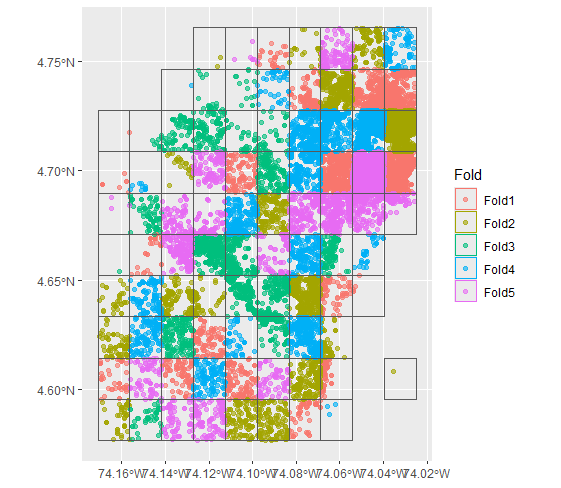
\includegraphics[width=0.75\linewidth]{Graficas/Validacion_Cruzada_Espacial.png}
\end{figure}





\end{document}
